%% 
%% Copyright 2019-2024 Elsevier Ltd
%% 
%% Version 2.4
%% 
%% This file is part of the 'CAS Bundle'.
%% --------------------------------------
%% 
%% It may be distributed under the conditions of the LaTeX Project Public
%% License, either version 1.2 of this license or (at your option) any
%% later version.  The latest version of this license is in
%%    http://www.latex-project.org/lppl.txt
%% and version 1.2 or later is part of all distributions of LaTeX
%% version 1999/12/01 or later.
%% 
%% The list of all files belonging to the 'CAS Bundle' is
%% given in the file `manifest.txt'.
%% 
%% Template article for cas-sc documentclass for 
%% single column output.

%\documentclass[a4paper,fleqn,longmktitle]{cas-sc}
\documentclass[a4paper,fleqn]{cas-sc}

\usepackage[utf8]{inputenc}

%\usepackage[numbers]{natbib}
%\usepackage[authoryear]{natbib}
\usepackage[export]{adjustbox}
\usepackage{amssymb}
\usepackage{fontawesome}
\usepackage[authoryear,longnamesfirst]{natbib}
\usepackage{tabularx}
\usepackage{subcaption}
\usepackage{tikz}
\usepackage{pgfplots}

\graphicspath{{figs/}}

%%%Author macros
\def\tsc#1{\csdef{#1}{\textsc{\lowercase{#1}}\xspace}}
\tsc{WGM}
\tsc{QE}
\tsc{EP}
\tsc{PMS}
\tsc{BEC}
\tsc{DE}
%%%

\pgfplotstableread{
	Participant Evaluation
	1 90.00
	2 95.00
	3 72.50
	4 60.00
	5 85.00
	6 67.50
	7 92.50
	8 67.50
	9 82.50
	10 85.00
	11 92.50
	12 87.50
}\susdata

\widowpenalty10000
\clubpenalty10000

% Valores calculados
\newcommand{\average}{81.46}
\newcommand{\stdev}{11.65}

\pgfmathsetmacro{\upperlimit}{\average+\stdev}
\pgfmathsetmacro{\lowerlimit}{\average-\stdev}


\newcommand{\utequrl}{https://www.uteq.edu.ec} % Define the URL macro

\begin{document}
	\let\WriteBookmarks\relax
	\def\floatpagepagefraction{1}
	\def\textpagefraction{.001}
	\shorttitle{Torddis: Detecting Distractions in Children's Academic Activities}
	\shortauthors{G. Guerrero-Ulloa et~al.}
	%\begin{frontmatter}
	
	\title [mode = title]{Torddis: A Real-Time IoT System for Detecting Distractions in Children's Home-Based  Academic Activities}                        
	\tnotemark[1]
	
	%\tnotetext[2]{The second title footnote which is a longer text matter to fill through the whole text width and overflow into another line in the footnotes area of the first page.}
	
	
	\author[1]{Gleiston Guerrero-Ulloa}[type=editor,orcid=000-0001-5990-2357,style=spanish]
	\ead{gguerrero@uteq.edu.ec}
	\ead[url]{\utequrl}
	
	\credit{Data curation, Methodology, Resources, Supervision, Validation, Visualization, Writing -- original draft, Writing -- review and editing,}
	
	\affiliation[1]{organization={Faculty of Engineering Sciences, State Technical University of Quevedo},
		addressline={Central Campus, Quito Avenue km. 1 1/2, on the way to Santo Domingo de los Tsáchilas}, 
		city={Quevedo},
		postcode={120301}, 
		state={Los Ríos},
		country={Ecuador}
	}
	
	\author[1]{Carlos Almeida-Dueñas}[type=editor,orcid=0000-0002-0959-922X,style=spanish]
	\ead{carlos.almeida2017@uteq.edu.ec}
	\ead[URL]{\utequrl}
	
	\credit{Conceptualization, Data curation, Formal analysis, Investigation, Software, Visualization}
	
	\author[1]{John Plazarte-Suárez}[orcid=0000-0001-5488-9982,style=spanish]
	%\fnmark[2]
	\ead{john.plazarte2017@uteq.edu.ec}
	\ead[URL]{\utequrl}
	
	\credit{Conceptualization, Data curation, Formal analysis, Investigation, Software, Visualization}
	
	\author[1]{Orlando Erazo-Moreta}[type=editor,orcid=0000-0001-5642-9920,
	style=spanish]
	%\fnmark[2]
	\ead{oerazo@uteq.edu.ec}
	\ead[URL]{\utequrl}
	
	\credit{Conceptualization, Data curation, Supervision, Validation, Visualization, Writing -- review and editing}
	
	\author[2]{Carlos Rodríguez-Domínguez}[
	orcid=0000-0001-5626-3115,
	style=spanish,
	%role=Supervisor and Validator
	]
	\cormark[1]
	\ead{carlosrodriguez@ugr.es}
	\ead[URL]{https://lsi.ugr.es/informacion/directorio-personal/carlos-rodriguez-dominguez}
	
	\credit{Data curation, Supervision, Validation, Visualization, Writing -- review and editing}
	
	\author[2]{Miguel J. Hornos}[orcid=0000-0001-5722-9816,style=spanish]
	%\fnmark[1,3]
	\ead{mhornos@ugr.es}
	\ead[URL]{https://lsi.ugr.es/informacion/directorio-personal/miguel-juan-hornos-barranco}
	
	\affiliation[2]{organization={Software Engineering Department, University of Granada},
		addressline={Calle Periodista Daniel Saucedo Aranda s/n}, 
		postcode={18071}, 
		postcodesep={}, 
		city={Granada},
		country={Spain}
	}
	
	\credit{Data curation, Supervision, Validation, Visualization, Writing -- review and editing}
	
	\cortext[cor1]{Corresponding author}
	%\cortext[cor2]{Principal corresponding author}
	
	%\nonumnote{Torddis is an innovative IoT system designed to monitor and improve student concentration at home, providing tutors with tools to detect distractions and maintain focus on school tasks.}
	
	%\fntext[fn1]{This document is the result of research conducted as part of teaching activities at the Technical State University of Quevedo, applying the findings from the Ph.D. thesis at the University of Granada.}
	
	\begin{abstract}
		Torddis es un sistema innovador diseñado para mitigar los efectos del ausentismo parental en el rendimiento académico mediante el uso de tecnologías de Inteligencia Artificial (IA) e Internet de las Cosas (IoT). El sistema monitorea en tiempo real las distracciones de los estudiantes en entornos domésticos, detectando expresiones faciales indicativas de distracción, objetos no autorizados y signos de somnolencia. Desarrollado utilizando la metodología TDDM4IoTS, Torddis integra una aplicación móvil con un dispositivo IoT para ofrecer a los tutores una herramienta práctica y eficiente para supervisar las actividades académicas en el hogar. Las evaluaciones de usabilidad realizadas por los tutores arrojaron una alta puntuación en la escala de usabilidad del sistema (SUS) del 81.46\%, lo que subraya la efectividad del sistema en mejorar la concentración de los estudiantes y proporcionar información valiosa para los padres. Aunque el sistema ha demostrado un potencial significativo, se han señalado recomendaciones para mejorar la calidad de la cámara. Torddis aspira a tener un impacto sustancial en la educación, sirviendo como un aliado robusto en el proceso de aprendizaje y ofreciendo prometedoras vías para futuros avances tecnológicos.
	\end{abstract}
	
	\begin{graphicalabstract}
		\includegraphics{figs/cas-grabs.pdf}
	\end{graphicalabstract}
	
	\begin{highlights}
		\item \textbf{Integración de Inteligencia Artificial e IoT:} Torddis utiliza tecnologías de IA e IoT para monitorizar en tiempo real las distracciones de los estudiantes en el hogar. El sistema identifica expresiones faciales indicativas de distracción, objetos no autorizados y signos de somnolencia, proporcionando una herramienta accesible y eficiente para la supervisión académica.
		\item \textbf{Metodología TDDM4IoTS:} Desarrollado siguiendo la metodología TDDM4IoTS, Torddis asegura la integración efectiva de una aplicación móvil y un dispositivo IoT, mejorando la supervisión académica y la concentración de los estudiantes. Esta metodología facilita el análisis del comportamiento de los niños mientras realizan tareas escolares de forma independiente en el hogar.
		\item \textbf{Evaluación de Usabilidad:} La usabilidad del sistema fue evaluada positivamente por los tutores, logrando una notable puntuación del 81.46\% en la escala de usabilidad del sistema (SUS). Esto resalta los beneficios del sistema para mejorar la concentración de los estudiantes y brindar apoyo informativo a los padres.
		\item \textbf{Alertas Visuales y Auditivas:} Los tutores enfatizaron la importancia de las alertas visuales y auditivas para mantener la atención de los estudiantes. El sistema incluye funciones que permiten la personalización de mensajes de audio y visuales, ayudando a mantener el enfoque de los niños durante las actividades académicas.
		\item \textbf{Impacto en la Educación:} Torddis promete un impacto significativo en la educación, posicionándose como un fuerte aliado en el aprendizaje y ofreciendo oportunidades para un mayor desarrollo. La integración de tecnologías avanzadas para la detección y respuesta en tiempo real a las distracciones subraya la relevancia de la innovación tecnológica en el ámbito educativo.
	\end{highlights}
	
	\begin{keywords}
		Internet of Things \sep
		Artificial Intelligence \sep
		Computer Vision \sep
		Distraction Monitoring \sep
		Student Concentration
	\end{keywords}
	
	\maketitle
	
	\section{Introducción}
	\label{seccion:Uno}
		Durante la última década, los estilos de vida acelerados y el aumento de la carga laboral han llevado a un incremento en el ausentismo parental durante las horas reservadas para las actividades de los estudiantes de primaria, lo cual ha resaltado la necesidad de soluciones tecnológicas que puedan suplir esta carencia de supervisión \cite{Abdul-Aziz2022,Ketsman2025Mapping}.
		
		Esta ausencia y falta de apoyo han demostrado afectar directamente el rendimiento académico de los jóvenes estudiantes. Los docentes han observado una disminución en los indicadores de rendimiento y disciplina, lo cual podría impactar negativamente la autoestima de los estudiantes y otros aspectos psicosociales. Además, la literatura sugiere que el apoyo emocional en el hogar es un pilar esencial para que los niños se concentren en sus estudios \citep{Abdul-Aziz2022}.
		
		La interferencia emocional influye no solo en el éxito educativo, sino que también impacta de manera significativa en todos los aspectos de la vida de los estudiantes \citep{Ake2023}. En este contexto, un entorno familiar que promueva la comunicación positiva y la interacción genuina puede mejorar el bienestar y las habilidades sociales de los estudiantes \citep{Navarro2024}. Sin embargo, para abordar de manera efectiva los desafíos asociados con la atención y la regulación emocional, es fundamental incorporar herramientas tecnológicas que integren Inteligencia Artificial (IA) e Internet de las Cosas (IoT). Estas tecnologías permiten monitorizar y medir las distracciones de los niños, proporcionando datos cruciales para la toma de decisiones orientadas a mejorar la atención y el aprendizaje \citep{Alvear-Puertas2017,Berrezueta-Guzman2021}.
		
		El uso de herramientas tecnológicas basadas en IA e IoT no solo contribuye al mejoramiento del rendimiento académico, sino que también fomenta habilidades de autorregulación en los estudiantes, esenciales para su desarrollo cognitivo y socioemocional \citep{Mohamed2018Implementing}. La retroalimentación que ofrecen estas tecnologías ayuda a los estudiantes a identificar sus distracciones y tomar acciones correctivas, lo que refuerza su capacidad para gestionar el tiempo y concentrarse en sus actividades. De esta manera, las herramientas tecnológicas se presentan como un recurso valioso para complementar la influencia positiva del entorno familiar y potenciar el aprendizaje autorregulado, creando un enfoque integral que abarca tanto el ámbito educativo como el personal \cite{Thinyane2016AUG}.
		
		La concentración de los estudiantes es un factor crucial que determina su capacidad para aprender y aplicar los conocimientos impartidos por los docentes. En un estudio realizado por \cite{Terraza2022}, se propone un sistema para monitorizar la atención de los estudiantes en un entorno de aprendizaje en línea utilizando algoritmos de visión por computadora. Los autores utilizan una Red Neuronal Recurrente (RNN) para identificar puntos de referencia faciales, que detectan si un estudiante mantiene una posición frontal hacia el dispositivo utilizado para asistir a una clase en línea. Su estudio resalta algunas limitaciones presentes en las propuestas actuales.
		
		Por otro lado, el trabajo de \cite{Berrezueta-Guzman2021} presenta un sistema robótico diseñado para interactuar con niños diagnosticados con Trastorno por Déficit de Atención e Hiperactividad (TDAH) para ayudarles a corregir hábitos poco saludables y comportamientos inapropiados asociados con el TDAH. Este sistema está orientado a niños diagnosticados con TDAH; sin embargo, a pesar de sus aspectos prometedores, cuando se aplica de manera general, puede perturbar a los niños sin tales condiciones. Además, este sistema carece de funciones de notificación, alerta o alarma para informar a sus tutores.
		
		En un esfuerzo por incluir la participación del tutor para mejorar el bienestar emocional de los niños, se introduce Torddis\footnote{Del latín \textbf{Tor}queo \textbf{d}iscerno \textbf{dis}cipulus'', que significa ``detección de desviación o cambio en la atención del estudiante.''}, como una solución que utiliza los avances tecnológicos para monitorizar el comportamiento de los estudiantes mientras realizan tareas escolares de forma independiente en sus hogares e informa a los tutores sobre cualquier desarrollo, para que puedan asegurar a sus hijos que no están solos. Además, Torddis está habilitado para reproducir sonidos que pueden ser mensajes personalizados de acuerdo con las preferencias de los usuarios.
		
		Para lograr sus objetivos, Torddis emplea algoritmos avanzados de visión por computadora y técnicas de aprendizaje profundo. El sistema incluye una aplicación móvil para tutores y un dispositivo IoT que facilita el análisis del comportamiento de los niños mientras realizan tareas escolares por su cuenta. Desarrollado utilizando la metodología TDDM4IoTS \citep{Guerrero-Ulloa2020TDDM4IoTS}, Torddis se destaca por su enfoque holístico. Permite a los tutores monitorizar y responder en tiempo real a signos de inatención. Las características clave incluyen la capacidad de detectar expresiones faciales que representan emociones fundamentales e identificar signos de somnolencia o el uso inadecuado de objetos durante las actividades educativas. Esta funcionalidad permite a los tutores alentar a sus hijos a mantener la concentración, utilizando tanto estímulos visuales como auditivos como motivadores \citep{Al-Gburi2023,Enadula2021,Terraza2022}.
		
		El sistema Torddis está diseñado para reforzar habilidades metacognitivas, como la gestión del tiempo y la concentración, esenciales en el aprendizaje moderno y en el contexto del aprendizaje autónomo. Su enfoque en la supervisión proactiva responde a la necesidad de apoyar a los niños durante una etapa crítica de desarrollo, proporcionando a los tutores una herramienta valiosa que complementa la supervisión tradicional en el hogar y contribuye a mejorar los resultados educativos de esta población.
		
		Este artículo está organizado en secciones que cubren diferentes aspectos de la implementación de la propuesta actual. La Sección \ref{seccion:Dos} se plantea la dimensión pedagógica del sistema TORDDIS. En La Sección \ref{seccion:Tres} revisa trabajos relacionados publicados en revistas internacionales de prestigio durante los últimos diez años. Estos trabajos están indexados en bases de datos como Web of Science (WoS), IEEE Xplore, ACM Digital Library y PubMed. La sección \ref{seccion:Cuatro} describe los materiales y métodos utilizados a lo largo del desarrollo y los procesos de evaluación del sistema. La Sección \ref{seccion:Cinco} presenta los principales resultados y discusión, y la Sección \ref{seccion:Seis} expone las conclusiones.
		
	\section{Dimensión Pedagógica de Torddis}
	\label{seccion:Dos}	
		Torddis no solo ofrece soluciones tecnológicas para monitorizar la concentración de los estudiantes, sino que también fomenta habilidades pedagógicas clave como la autorregulación y el aprendizaje autónomo. Al proporcionar retroalimentación inmediata y personalizada, el sistema ayuda a los estudiantes a desarrollar estrategias efectivas para gestionar su tiempo y su atención, competencias esenciales en el aprendizaje moderno \cite{Loh2025Plugging}
		
		La autorregulación, entendida como la capacidad de los estudiantes para gestionar y evaluar su propio proceso de aprendizaje, se convierte en una competencia esencial en el desarrollo educativo \cite{Palioura2025Storylling}. Diversas investigaciones, que abarcan desde la implementación de lenguajes de programación visual en la educación primaria \citep{SaezLopez2016Visual} hasta la incorporación de metodologías activas en el aula \citep{Mohamed2018Implementing}, resaltan que los entornos tecnológicos y las estrategias pedagógicas pueden promover significativamente la autorregulación en los estudiantes.
		
		Estos enfoques permiten a los niños interactuar de forma autónoma y reflexiva, generando hábitos que fortalecen su capacidad para mantener la concentración y gestionar su tiempo y sus recursos de manera efectiva. En este contexto, Torddis se presenta no solo como una herramienta de monitorización, sino como un aliado pedagógico que contribuye al desarrollo de habilidades de autorregulación y refuerza el rol del tutor o profesor en el proceso de aprendizaje.
		
		\subsection{Importancia de la autorregulación en el aprendizaje}
			El desarrollo de la autorregulación en el aprendizaje resulta fundamental para la autonomía académica, ya que permite a los estudiantes tomar control sobre su propio proceso de aprendizaje, estableciendo metas, evaluando sus avances y ajustando sus estrategias. La investigación de \cite{Taber2024Developing} ejemplifica cómo la autorregulación es esencial en disciplinas que demandan habilidades de gestión autónoma, permitiendo a los estudiantes monitorizar y mejorar continuamente su rendimiento.
			
			Asimismo, los entornos educativos pueden fomentar esta competencia mediante metodologías activas y el uso de tecnologías. Por ejemplo, el uso de lenguajes de programación visual, como Scratch, en la educación básica ayuda a los estudiantes a experimentar y tomar decisiones, desarrollando así habilidades de autorregulación a través de la exploración y el control personal de sus actividades de aprendizaje. El aula invertida apoyada por sistemas de tutoría inteligente, descrito en el trabajo de \cite{Mohamed2018Implementing} permite a los estudiantes trabajar de forma independiente fuera del aula y recibir retroalimentación inmediata, promoviendo un proceso de aprendizaje autorregulado y adaptativo.
			
			Finalmente, el uso de dinámicas de juego colaborativo, como  exploran \cite{Echeverria2011AFramework} contribuye al desarrollo de competencias de autorregulación en un entorno lúdico. Estas experiencias, al involucrar al estudiante en la toma de decisiones y el manejo de objetivos, consolidan habilidades de autocontrol y manejo de tiempo esenciales en el aprendizaje autónomo.
			
			Estas investigaciones destacan que el desarrollo de la autorregulación mediante enfoques tecnológicos y pedagógicos no solo optimiza el aprendizaje autónomo, sino que también prepara a los estudiantes para enfrentar de forma reflexiva y adaptativa los retos de su proceso educativo.
			
		\subsection{Torddis y su contribución a la supervisión del aprendizaje autónomo en el hogar}		
			El sistema Torddis está diseñado para apoyar el aprendizaje autónomo en los estudiantes a través de herramientas tecnológicas que permiten la supervisión y la monitorización en tiempo real de la concentración durante sus actividades académicas en el hogar. Estudios recientes han demostrado que herramientas basadas en IA, como ChatGPT, pueden facilitar experiencias de aprendizaje autodirigido y personalizadas, fomentando la autonomía y mejorando los resultados educativos \cite{Li2024Systematic}.
			
			Así mismo, estudios previos destacan que el aprendizaje personalizado fomenta la motivación intrínseca y la autorregulación en los estudiantes más jóvenes, mejorando su desempeño académico \cite{Ackermans2025Young}. Mediante el análisis de expresiones faciales, la detección de objetos y el reconocimiento de estados de somnolencia, el sistema ayuda a los estudiantes a mantener el enfoque en sus tareas escolares, permitiéndoles desarrollar habilidades esenciales de autorregulación como la atención sostenida, la gestión del tiempo y el autocontrol.
			
			Una característica clave de Torddis es su capacidad para detectar distracciones y emitir alertas visuales y sonoras, brindando a los estudiantes una retroalimentación inmediata que los ayuda a redirigir su atención hacia las actividades académicas. Esta retroalimentación en tiempo real refuerza el proceso de autorreflexión y autoevaluación, aspectos cruciales en la autorregulación del aprendizaje. Además, al incorporar a los tutores en el proceso, Torddis establece un entorno de aprendizaje colaborativo donde los padres pueden observar y analizar los patrones de comportamiento de sus hijos, lo que permite una intervención oportuna en caso de que se identifiquen barreras para el aprendizaje.
			
			La capacidad de Torddis para registrar y visualizar datos históricos de las distracciones de los estudiantes y otros parámetros relevantes también permite un seguimiento constante y la identificación de áreas específicas en las que el estudiante podría mejorar su autorregulación. Este enfoque integral no solo optimiza el tiempo y esfuerzo del estudiante, sino que también proporciona a los tutores una herramienta confiable para apoyar el proceso de aprendizaje en ausencia de supervisión constante, promoviendo una educación que fomente la autonomía y la autogestión en el estudiante.
		
		\subsection{Relación de Torddis con las competencias digitales}
			Torddis se presenta como una herramienta educativa que promueve activamente el desarrollo de competencias digitales entre los estudiantes. En la era de la digitalización, los estudiantes requieren habilidades que les permitan interactuar eficazmente con herramientas tecnológicas para maximizar sus oportunidades de aprendizaje y, al mismo tiempo, adquirir habilidades críticas para el futuro. El sistema apoya este desarrollo al facilitar un entorno en el cual los estudiantes pueden participar en actividades interactivas y autónomas, permitiéndoles mejorar sus competencias en la resolución de problemas y en el uso efectivo de la tecnología educativa.
			
			Implementaciones como el aula invertida, donde los estudiantes acceden a contenido digital fuera del horario de clases y emplean las horas presenciales para actividades prácticas, han demostrado ser eficaces en el aumento de la motivación y del compromiso del estudiante al situarlos en el centro del proceso de aprendizaje, promoviendo un ambiente de colaboración y un aprendizaje autodirigido, que son componentes esenciales de las competencias digitales \citep{Mohamed2018Implementing}. Además, estudios en entornos de aprendizaje colaborativo evidencian que el uso de juegos digitales y plataformas de aprendizaje programado contribuyen al desarrollo de habilidades digitales y colaborativas al proporcionar escenarios de aprendizaje basados en la interacción con herramientas digitales \citep{Echeverria2011AFramework}, algo que Torddis también facilita a través de su diseño orientado a la interacción y la supervisión en tiempo real.
			
			\cite{Coffman2024Developing} mencionan que en el ámbito de la educación en enfermería, la autorregulación ha sido una estrategia fundamental para fomentar la autodisciplina y el uso efectivo de tecnologías digitales en el aprendizaje, demostrando que los estudiantes mejoran su rendimiento académico y su adaptabilidad a entornos clínicos y digitales al incorporar estrategias de autorregulación que Torddis puede fomentar desde edades tempranas mediante supervisión y retroalimentación constante. Por lo tanto, Torddis se alinea con las mejores prácticas de pedagogía moderna, apoyando un aprendizaje autónomo y digitalmente competente, necesario para responder a las demandas del siglo XXI.
	
	\section{Related Works}
	\label{seccion:Tres}
		La literatura sobre el uso de tecnologías para la detección y corrección de distracciones en estudiantes es limitada, especialmente en lo que respecta a la integración de tecnologías IoT con fines pedagógicos. Los estudios previos han abordado aplicaciones tecnológicas en la monitorización de niños, pero pocos han explorado cómo estas tecnologías pueden ser utilizadas para proporcionar retroalimentación inmediata que fomente la autorregulación del aprendizaje y mejore los resultados educativos en contextos no formales.El proceso de revisión del estado del arte siguió la metodología descrita en el esquema de la Figura \ref{fig:LRS}.
		
		\begin{figure}[h]
			\includegraphics[width=\textwidth]{Figure_1}
			\caption{Literature Review Scheme.}
			\label{fig:LRS}
		\end{figure}   
		
		\subsection{Research Questions}
			Este artículo explora el tema crítico de la detección de distracciones en los estudiantes mientras realizan tareas escolares de forma independiente. Con el aumento de las herramientas digitales de educación y la necesidad de estrategias de aprendizaje efectivas, comprender cómo las distracciones afectan el rendimiento estudiantil se ha vuelto fundamental. Las siguientes preguntas de investigación tienen como objetivo guiar una revisión exhaustiva de los trabajos relacionados e informar el desarrollo de soluciones tecnológicas que mejoren la concentración y los resultados educativos de los niños. Estas preguntas ayudarán a identificar los métodos y tecnologías más efectivos para monitorizar y mitigar las distracciones durante las actividades educativas.
		
			\begin{itemize}
				\item ¿Cuáles son los parámetros de distracción que deberían monitorizarse en los niños durante la realización de sus tareas escolares?
				\item ¿Qué modelos computacionales son adecuados para detectar el comportamiento de los niños mientras realizan tareas escolares?
				\item ¿Qué algoritmos enfocados en la detección de distracciones podrían ser utilizados en el desarrollo de la propuesta?
				\item ¿Qué tecnologías de hardware y software podrían emplearse para desarrollar un dispositivo prototipo que apoye la concentración de los niños durante las actividades escolares?
			\end{itemize}
			%\unskip
		
		\subsection{Estrategias de Búsqueda}
			Una vez definidas las preguntas de investigación, se seleccionaron las palabras clave relevantes para recuperar trabajos publicados en las principales bases de datos científicas más pertinentes para este campo de investigación. Estas palabras clave se utilizaron para formar la cadena de búsqueda, la cual fue adaptada específicamente para cada base de datos científica seleccionada. La cadena de búsqueda utilizada fue: ("distracción") AND ("niño" OR "niños" OR "estudiante" OR "tarea escolar" OR "deberes") AND ("reconocimiento de objetos" OR "reconocimiento facial" OR "reconocimiento de gestos").
		
			Las bases de datos utilizadas incluyeron ACM, IEEE Xplorer, PubMed, Scopus y Web of Science. Además, se empleó Google Scholar para ampliar los resultados y así minimizar la posibilidad de excluir documentos importantes como trabajos relacionados. La Tabla \ref{tab:Results} muestra la búsqueda inicial en estas bases de datos y en Google Scholar. Tras un análisis individual de los documentos encontrados en las bases de datos, se consideró que el 82\% de ellos eran relevantes. En contraste, de los resultados del motor de búsqueda académico, se revisaron los primeros 500 resultados en orden de relevancia, con 6 (y duplicados 16) de los primeros 300 considerados pertinentes. Los siguientes 200 resultados no estaban relacionados con las preguntas de investigación de este estudio, lo que llevó a asumir que no se encontrarían más documentos relevantes.
		
			\begin{table}[H] 
				\caption{Resultados de la búsqueda de trabajos relacionados.\label{tab:Results}}
				\begin{tabularx}{0.90\textwidth}{>{\centering\arraybackslash}X >{\centering\arraybackslash}X >{\centering\arraybackslash}X >{\centering\arraybackslash}X >{\centering\arraybackslash}X}
					\toprule
					\textbf{Base de Datos/Motor de Búsqueda}	& \textbf{Resultados Preliminares} & \textbf{Duplicados} & \textbf{Análisis de Título y Resumen} & \textbf{Resultados Finales}\\
					\midrule
					ACM 			& 	1 		& 	0 	& 	1	&	1\\
					IEEE Xplorer	& 	3		&  	0 	& 	2	&	2\\
					PubMed			&  	1 		& 	0 	& 	0	&	0\\
					Scopus			&  	22 		& 	3 	& 	19	&	15\\
					Web of Science	&  	8 		& 	6 	& 	2	&	2\\
					Google Scholar	&  	15,400 (primeros 500) 	& 	19 	& 	16	&	6\\
					\bottomrule
				\end{tabularx}
			\end{table}
		
		%\subsection{Análisis de la Literatura}			
			%En la literatura científica sobre tecnologías aplicadas a los sectores de la educación y el cuidado infantil, existen diversos enfoques centrados en el uso de IA, IoT y técnicas de visión por computadora para mejorar el aprendizaje y la monitorización del comportamiento. Además, otros estudios han integrado estas tecnologías para facilitar la autorregulación del aprendizaje, mejorar la concentración y fomentar el compromiso académico en diversos grupos de estudiantes.
		
		%\subsubsection{Monitorización del Comportamiento}
			%Investigaciones como las de \cite{Akter2021}, \cite{Albrecht2014}, \cite{Berrezueta-Guzman2021}, \cite{Pelc2006}, \cite{VilliersRader2021}, \cite{Warren2015Brief}, \cite{Washington2016AWereable} exploran aplicaciones que van desde el diagnóstico temprano del trastorno del espectro autista (TEA) hasta la mejora en el reconocimiento de emociones en niños con trastornos de déficit de atención (TDAH). Estos estudios utilizan tecnologías avanzadas como la inteligencia artificial (IA) y dispositivos conectados para analizar y responder a comportamientos específicos de los niños en entornos controlados o cotidianos.
		
			%Por ejemplo, \cite{Akter2021} emplea el aprendizaje por transferencia para diagnosticar el TEA mediante el reconocimiento facial. De manera similar, \cite{Pelc2006} se enfoca en reconocer emociones en niños con TDAH mediante fotografías validadas, mientras que \cite{Albrecht2014} investiga las estrategias de búsqueda visual en niños con TEA. \cite{Berrezueta-Guzman2021} evalúa el uso de un asistente robótico para apoyar actividades escolares de niños con TDAH, y \cite{VilliersRader2021} examina cómo los gestos pueden dirigir la atención hacia las relaciones entre palabras y objetos en niños con TEA.
		
			%Estudios adicionales de \cite{Boumiza2017}, \cite{DaCosta2023}, \cite{Enadula2021}, \cite{Farsani2020}, \cite{Hachad2020}, \cite{James2019},  \cite{Kulkarni2023}, \cite{Kumar2024Zoom}, \cite{Muller2018ArchnSmile}, \cite{Narkhede2023}, y \cite{Ozdamli2022} también abordan problemas relacionados con la seguridad, el compromiso y la interacción mediante tecnologías de monitorización. Por ejemplo, \cite{Hachad2020} y \cite{James2019} emplean el reconocimiento facial para monitorizar la seguridad de los estudiantes en autobuses escolares y la asistencia en aulas, respectivamente. Asimismo, \cite{Ozdamli2022} utiliza tecnologías de visión por computadora para reconocer emociones y detectar trampas durante exámenes en línea.
		
			%Además, \cite{Campbell2015Using} y \cite{Ucar2022Recognizing} presentan sistemas diseñados para monitorizar distracciones en tiempo real. Por ejemplo, \cite{Campbell2015Using} utiliza imágenes multiespectrales para identificar distracciones causadas por dispositivos móviles, mientras que \cite{Ucar2022Recognizing} emplea reconocimiento facial y estimación de la postura de la cabeza para evaluar el compromiso de los estudiantes en clases virtuales. Por otro lado, trabajos como los de \cite{Argel2023Intellitell}, \cite{Erazo2016Easing}, y \cite{Nguyen2019} también se orientan a la evaluación del comportamiento mediante tecnologías avanzadas como YOLOv3 para la monitorización de respuestas en tiempo real y ajustes dinámicos en métodos de enseñanza.
		
			%Finalmente, estudios como \cite{Boumiza2017} y \cite{DaCosta2023} exploran la monitorización en contextos de transporte escolar y tutorías automatizadas en ciudades inteligentes, destacando el uso del reconocimiento facial para personalizar la experiencia educativa y mejorar la seguridad.
			
		%\subsubsection{Tecnología para el Aprendizaje Autónomo}
			%Otros estudios se enfocan en promover la autorregulación, la concentración y el compromiso académico, integrando tecnologías que apoyan el aprendizaje autónomo en diversos contextos. Por ejemplo, \cite{Bembich2016Future} investiga el uso de tecnologías digitales para futuros educadores, proporcionando estrategias de autorregulación para gestionar distracciones. De manera similar, \cite{Peters2003Self} examina cómo entornos hipertextuales pueden mejorar el control volicional y la gestión de distracciones en el aprendizaje digital autónomo.
		
			%\cite{Roberts2020Task} analiza cómo los estudiantes de secundaria utilizan registros digitales para autorregularse y reflexionar sobre su progreso académico. Por otro lado, \cite{Adcroft2018Developing} combina tecnologías con prácticas de manejo del tiempo y mindfulness para ayudar a los estudiantes a mejorar su concentración y autorregulación en tareas diarias.
		
			%Trabajos como \cite{Salter2014Exploring} y \cite{Palmer2022impact} integran tecnologías y plataformas para monitorizar y evaluar habilidades de autorregulación. Mientras que \cite{Salter2014Exploring} adopta un enfoque integral a nivel escolar, \cite{Palmer2022impact} se centra en la enseñanza híbrida sincrónica en educación farmacéutica.
		
			%Por otro lado, \cite{Muljana2022Instructional} y \cite{Wang2022Empowering} abordan estrategias específicas para fomentar la autorregulación. Mientras que \cite{Muljana2022Instructional} analiza cómo profesionales educativos emplean redes sociales para desarrollar su aprendizaje autorregulado, \cite{Wang2022Empowering} investiga la reducción de distracciones digitales en estudiantes universitarios mediante habilidades de autorregulación.
		
			%Además, \cite{Hartley2022Smartphone} y \cite{Labar2019Interplay} examinan el impacto del uso de dispositivos móviles en la atención y el multitasking. Mientras que \cite{Labar2019Interplay} adopta un enfoque psicológico para analizar la percepción del tiempo, \cite{Hartley2022Smartphone} se enfoca en cómo el uso del teléfono inteligente afecta directamente las habilidades de autorregulación.
		
			%Estos trabajos reflejan un enfoque diverso hacia la autorregulación y la mejora del aprendizaje autónomo, empleando estrategias tecnológicas para reducir distracciones, mejorar el control volicional y fomentar el compromiso académico.
		
		\subsection{Análisis de la Literatura}			
			En la literatura científica sobre tecnologías aplicadas a los sectores de la educación y el cuidado infantil, existen diversos enfoques centrados en el uso de IA, IoT y técnicas de visión por computadora para mejorar el aprendizaje y la monitorización del comportamiento. Además, otros estudios han integrado estas tecnologías para facilitar la autorregulación del aprendizaje, mejorar la concentración y fomentar el compromiso académico en diversos grupos de estudiantes.
			
			\subsubsection{Monitorización del Comportamiento}
				Investigaciones como las de \cite{Akter2021}, \cite{Albrecht2014}, \cite{Berrezueta-Guzman2021}, \cite{Pelc2006}, \cite{VilliersRader2021}, \cite{Warren2015Brief}, \cite{Washington2016AWereable} exploran aplicaciones que van desde el diagnóstico temprano del trastorno del espectro autista (TEA) hasta la mejora en el reconocimiento de emociones en niños con trastornos de déficit de atención (TDAH). Estos estudios utilizan tecnologías avanzadas como la inteligencia artificial (IA) y dispositivos conectados para analizar y responder a comportamientos específicos de los niños en entornos controlados o cotidianos.
				
				Por ejemplo, \cite{Akter2021} emplea el aprendizaje por transferencia para diagnosticar el TEA mediante el reconocimiento facial. De manera similar, \cite{Pelc2006} se enfoca en reconocer emociones en niños con TDAH mediante fotografías validadas, mientras que \cite{Albrecht2014} investiga las estrategias de búsqueda visual en niños con TEA. \cite{Berrezueta-Guzman2021} evalúa el uso de un asistente robótico para apoyar actividades escolares de niños con TDAH, y \cite{VilliersRader2021} examina cómo los gestos pueden dirigir la atención hacia las relaciones entre palabras y objetos en niños con TEA.
				
				Estudios adicionales de \cite{Boumiza2017}, \cite{DaCosta2023}, \cite{Enadula2021}, \cite{Farsani2020}, \cite{Hachad2020}, \cite{James2019},  \cite{Kulkarni2023}, \cite{Kumar2024Zoom}, \cite{Muller2018ArchnSmile}, \cite{Narkhede2023}, y \cite{Ozdamli2022} también abordan problemas relacionados con la seguridad, el compromiso y la interacción mediante tecnologías de monitorización. Por ejemplo, \cite{Hachad2020} y \cite{James2019} emplean el reconocimiento facial para monitorizar la seguridad de los estudiantes en autobuses escolares y la asistencia en aulas, respectivamente. Asimismo, \cite{Ozdamli2022} utiliza tecnologías de visión por computadora para reconocer emociones y detectar trampas durante exámenes en línea.
				
				Además, \cite{Campbell2015Using} y \cite{Ucar2022Recognizing} presentan sistemas diseñados para monitorizar distracciones en tiempo real. Por ejemplo, \cite{Campbell2015Using} utiliza imágenes multiespectrales para identificar distracciones causadas por dispositivos móviles, mientras que \cite{Ucar2022Recognizing} emplea reconocimiento facial y estimación de la postura de la cabeza para evaluar el compromiso de los estudiantes en clases virtuales. Por otro lado, trabajos como los de \cite{Argel2023Intellitell}, \cite{Erazo2016Easing}, y \cite{Nguyen2019} también se orientan a la evaluación del comportamiento mediante tecnologías avanzadas como YOLOv3 para la monitorización de respuestas en tiempo real y ajustes dinámicos en métodos de enseñanza.
				
				Finalmente, estudios como \cite{Boumiza2017} y \cite{DaCosta2023} exploran la monitorización en contextos de transporte escolar y tutorías automatizadas en ciudades inteligentes, destacando el uso del reconocimiento facial para personalizar la experiencia educativa y mejorar la seguridad.
				
			\subsubsection{Tecnología para el Aprendizaje Autónomo}
				Otros estudios se enfocan en promover la autorregulación, la concentración y el compromiso académico, integrando tecnologías que apoyan el aprendizaje autónomo en diversos contextos. Por ejemplo, \cite{Bembich2016Future} investiga el uso de tecnologías digitales para futuros educadores, proporcionando estrategias de autorregulación para gestionar distracciones. De manera similar, \cite{Peters2003Self} examina cómo entornos hipertextuales pueden mejorar el control volicional y la gestión de distracciones en el aprendizaje digital autónomo.
				
				\cite{Roberts2020Task} analiza cómo los estudiantes de secundaria utilizan registros digitales para autorregularse y reflexionar sobre su progreso académico. Por otro lado, \cite{Adcroft2018Developing} combina tecnologías con prácticas de manejo del tiempo y mindfulness para ayudar a los estudiantes a mejorar su concentración y autorregulación en tareas diarias.
				
				Trabajos como \cite{Salter2014Exploring} y \cite{Palmer2022impact} integran tecnologías y plataformas para monitorizar y evaluar habilidades de autorregulación. Mientras que \cite{Salter2014Exploring} adopta un enfoque integral a nivel escolar, \cite{Palmer2022impact} se centra en la enseñanza híbrida sincrónica en educación farmacéutica.
				
				Por otro lado, \cite{Muljana2022Instructional} y \cite{Wang2022Empowering} abordan estrategias específicas para fomentar la autorregulación. Mientras que \cite{Muljana2022Instructional} analiza cómo profesionales educativos emplean redes sociales para desarrollar su aprendizaje autorregulado, \cite{Wang2022Empowering} investiga la reducción de distracciones digitales en estudiantes universitarios mediante habilidades de autorregulación.
				
				Además, \cite{Hartley2022Smartphone} y \cite{Labar2019Interplay} examinan el impacto del uso de dispositivos móviles en la atención y el multitasking. Mientras que \cite{Labar2019Interplay} adopta un enfoque psicológico para analizar la percepción del tiempo, \cite{Hartley2022Smartphone} se enfoca en cómo el uso del teléfono inteligente afecta directamente las habilidades de autorregulación.
				
				Estos trabajos reflejan un enfoque diverso hacia la autorregulación y la mejora del aprendizaje autónomo, empleando estrategias tecnológicas para reducir distracciones, mejorar el control volicional y fomentar el compromiso académico.
				
			\subsubsection{Comparación de la Literatura Revisada con TORDDIS}
				El análisis de la literatura evidencia un progreso significativo en el uso de tecnologías avanzadas para abordar problemáticas educativas y de cuidado infantil. Sin embargo, TORDDIS sobresale como una solución integral, combinando IoT, visión por computadora e inteligencia artificial para ofrecer supervisión adaptativa y proactiva en diversos entornos. A continuación, se detalla cómo TORDDIS supera las limitaciones observadas en las referencias revisadas.
				
				En el ámbito de la monitorización del comportamiento, trabajos como \cite{Akter2021}, \cite{Pelc2006}, y \cite{Albrecht2014} emplean reconocimiento facial y análisis visual para diagnosticar TEA y TDAH. Aunque estos enfoques son valiosos para entender patrones conductuales, carecen de intervención en tiempo real, algo que TORDDIS implementa mediante alertas proactivas que redirigen la atención del estudiante. Por otro lado, estudios como \cite{Campbell2015Using}, \cite{Ucar2022Recognizing}, y \cite{Argel2023Intellitell} se centran en identificar distracciones, pero no incluyen capacidades de adaptación al entorno doméstico, un contexto menos estructurado que TORDDIS aborda de manera eficaz.
				
				Adicionalmente, investigaciones como \cite{Berrezueta-Guzman2021}, \cite{VilliersRader2021}, y \cite{Washington2016AWereable} introducen tecnologías portátiles y robóticas para niños con trastornos del desarrollo. Aunque estas propuestas personalizan el apoyo en el aula, no extienden su alcance al hogar ni permiten una supervisión continua sin intervención constante de un adulto. Por su parte, trabajos como \cite{Muller2018ArchnSmile} y \cite{Nguyen2019} se enfocan en actividades lúdicas mediante reconocimiento facial, pero su aplicación está restringida al entretenimiento, mientras que TORDDIS equilibra actividades educativas con estrategias para fomentar la atención.
				
				En términos de seguridad y personalización educativa, estudios como \cite{Hachad2020}, \cite{James2019}, y \cite{Boumiza2017} aplican reconocimiento facial para tareas administrativas como la asistencia y la seguridad en el transporte escolar. Sin embargo, no abordan la integración pedagógica ni la monitorización adaptativa del comportamiento estudiantil. Por otro lado, sistemas como los de \cite{DaCosta2023}, \cite{Kumar2024Zoom}, y \cite{Narkhede2023} emplean tecnologías para detectar emociones y atención durante actividades académicas, pero no logran integrar detección de objetos distractores ni respuestas proactivas como las de TORDDIS.
				
				Respecto a tecnologías para el aprendizaje autónomo, trabajos como \cite{Bembich2016Future}, \cite{Roberts2020Task}, y \cite{Peters2003Self} se centran en fomentar la autorregulación a través de herramientas digitales. Por otro lado, \cite{Muljana2022Instructional} analiza cómo diseñadores instruccionales emplean redes sociales para promover la autorregulación, pero estas estrategias dependen completamente del compromiso del usuario, careciendo de capacidades automatizadas para redirigir la atención. En contraste, \cite{Palmer2022impact}, \cite{Adcroft2018Developing}, y \cite{Salter2014Exploring} introducen prácticas pedagógicas como mindfulness y enseñanza híbrida, pero tampoco incorporan tecnologías avanzadas como las de TORDDIS para intervenir directamente en el proceso de aprendizaje.
				
				Otro contexto en que se han aplicado tecnologías es en el ámbito de multitarea y distracciones digitales, investigaciones como \cite{Hartley2022Smartphone}, \cite{Labar2019Interplay}, y \cite{Farsani2020} analizan el impacto de los dispositivos móviles en la atención y el compromiso académico. Aunque estas propuestas destacan problemas clave, TORDDIS sobresale al detectar automáticamente distracciones generadas por dispositivos y aplicar estrategias correctivas inmediatas. Además, estudios como \cite{Erazo2016Easing} y \cite{Wang2022Empowering} abordan distracciones digitales desde perspectivas gestuales y pedagógicas, respectivamente, pero no ofrecen intervención automatizada en tiempo real.
				
				Por último, referencias como \cite{Kulkarni2023 }, \cite{Enadula2021}, \cite{Ozdamli2022}, y \cite{Warren2015Brief} destacan el uso de tecnologías avanzadas para la \textit{interacción educativa y la detección de emociones}. Sin embargo, estas investigaciones no consideran la multidimensionalidad que TORDDIS introduce al combinar análisis emocional, cognitivo y contextual para intervenir de manera efectiva en entornos académicos y domésticos.
				
			\subsection{Conclusión}
				Finalmente se puede concluir que, mientras los trabajos revisados ofrecen avances significativos en áreas específicas, TORDDIS se posiciona como una solución integrada que no solo supera las limitaciones técnicas de los sistemas actuales, sino que también atiende las necesidades dinámicas de los entornos educativos y de cuidado infantil con un enfoque proactivo y adaptativo.
			
	\section{Materiales y Métodos}
	\label{seccion:Cuatro}
		La presente sección describe en detalle los procedimientos, herramientas y metodologías empleadas en el diseño, desarrollo y evaluación del sistema Torddis. Este sistema combina tecnologías avanzadas de Internet de las Cosas (IoT) e Inteligencia Artificial (IA) para monitorizar y mejorar la concentración de los estudiantes en actividades académicas realizadas en el hogar. El enfoque metodológico estuvo guiado por la metodología TDDM4IoTS, permitiendo un desarrollo iterativo y enfocado en la calidad técnica y pedagógica.
		
		A través de este apartado, se exponen las características de los participantes, el diseño experimental, las técnicas utilizadas para la validación de instrumentos y análisis de datos, así como los aspectos técnicos del sistema. Además, se destacan las medidas adoptadas para reducir sesgos, asegurar la confiabilidad de los resultados y responder a las necesidades educativas y tecnológicas de los usuarios finales. Finalmente, se reconocen las limitaciones del estudio y se justifica el impacto pedagógico del sistema en el desarrollo de habilidades de autorregulación y aprendizaje autónomo.
		
		\subsection{Participantes y Contexto del Estudio}
			El estudio incluyó la participación de 12 niños con su respectivo tutor, seleccionados mediante un muestreo por conveniencia. Los niños tenían edades comprendidas entre los 7 y 12 años, cursando estudios primarios y secundarios. Los tutores, de entre 25 y 65 años, presentaban niveles de educación primaria y secundaria. Los participantes residen en sectores urbanos y rurales con servicios básicos (electricidad, agua potable, Internet y telefonía móvil).
				
			El criterio de selección garantizó que los hogares contaran con acceso a Internet en el domicilio (WiFi o datos móviles) y datos móviles en el Smartphone del tutor, condiciones necesarias para implementar el sistema. Este enfoque asegura que los participantes representan el perfil de los usuarios potenciales de Torddis: familias con tutores ocupados en actividades dentro y fuera del hogar, responsables de niños en edad escolar que necesitan supervisión directa.
				
			La representatividad de la muestra se considera aceptable al trabajar con usuarios reales del sistema y cumplir con criterios de inclusión definidos. La selección por conveniencia es adecuada en investigaciones preliminares como esta, permitiendo obtener una muestra significativa pese a la limitada disposición de colaboración de algunas familias \citep{DiPietro2025Meta}.
				
		\subsection{Proceso Experimental y Validación de Instrumentos}
			El proceso experimental se llevó a cabo en dos etapas:
				
			\paragraph{Entorno simulado:} Diseñado para evaluar la usabilidad y rendimiento del sistema. Durante esta fase, los tutores usaron Torddis durante 30 minutos en un entorno controlado, donde se verificaron todas las funcionalidades del sistema. Se emplearon cuestionarios SUS y preguntas abiertas para recopilar datos sobre la experiencia del usuario.
			
			\paragraph{Entorno real:} Diseñado para evaluar la efectividad del sistema. Esta fase duró una semana, considerando que solo existía un prototipo. Se utilizó un cuestionario con escala de Likert para medir la percepción de los tutores sobre la utilidad y efectividad de Torddis (ver \ref{Appendix:Effectivity}), incluyendo preguntas sobre atracción del dispositivo, precisión de las notificaciones, y su impacto en la autorregulación y concentración de los niños \citep{Ackermans2025Young}.
				
			La validez de los instrumentos fue garantizada mediante la revisión y validación por investigadores con experiencia, quienes aseguraron la claridad de las preguntas y su adecuación al propósito del estudio. Además, los datos generados por el sistema (e.g., detección de objetos, alertas) fueron corroborados manualmente para garantizar su precisión \citep{Wang2025Development}. Además, se calculó el Alpha de Cronbach \citep{Forero2024Cronbach} para medir la consistencia interna entre las afirmaciones.
			
		\subsection{Aleatorización y Sesgos}
			No se implementó un proceso de aleatorización debido a la naturaleza del muestreo por conveniencia. Sin embargo, se tomaron medidas para minimizar sesgos, como \citep{Huang2025How}:
			
			\begin{itemize}
				\item Explicación detallada de las preguntas del cuestionario antes de su llenado.
				\item Garantía de anonimato y confidencialidad de las respuestas.
				\item Aplicación del cuestionario sin la presencia de los investigadores para evitar influencia en las respuestas.
			\end{itemize}
				
			Reconocemos que podrían existir sesgos relacionados con la cercanía de los investigadores a los participantes, lo que podría influir en las respuestas de los cuestionarios \citep{DiPietro2025Meta}.
			
		\subsection{Análisis Estadístico}
			Los datos obtenidos fueron analizados utilizando métodos descriptivos y correlacionales. Para las evaluaciones de usabilidad (SUS), se calculó un puntaje promedio para determinar la aceptación del sistema. En la fase real, se empleó análisis correlacional para explorar relaciones entre las variables medidas (e.g., percepción del tutor sobre la mejora en la autorregulación y concentración de los niños) \citep{Wang2025Development}.
				
			El análisis estadístico permite identificar patrones significativos en el uso del sistema, justificando su validez en contextos similares. Los métodos empleados son apropiados para estudios piloto, donde el tamaño de la muestra limita el uso de pruebas inferenciales más robustas.
			
		\subsection{Limitaciones y Generalización}
			El estudio presenta ciertas limitaciones:
				
			\begin{enumerate}
				\item La muestra se limita a un grupo pequeño de participantes seleccionados por conveniencia, lo que podría no representar otros contextos sociodemográficos o tecnológicos.
				\item La duración de la fase real (una semana) no permite evaluar el impacto a largo plazo del sistema en habilidades como la autorregulación.
				\item La disponibilidad de un único prototipo restringió la simultaneidad del uso por varios participantes.
			\end{enumerate}
		
			Estas limitaciones son comunes en investigaciones que exploran el impacto de tecnologías educativas en contextos iniciales o pilotos. Estudios previos han destacado que la generalización de los resultados en intervenciones tecnológicas depende en gran medida de las características específicas de la población y del entorno en el que se implementan. Por ejemplo, una meta-análisis reciente sobre los efectos de la tecnología en estudiantes desfavorecidos resalta cómo las variaciones en el acceso a recursos y las condiciones contextuales pueden influir significativamente en los resultados obtenidos, sugiriendo la necesidad de diseñar futuros estudios que incluyan una muestra más amplia y diversa para aumentar la representatividad de los hallazgos \citep{DiPietro2025Meta}.
			
		\subsection{Desarrollo de TORDDIS}
			El desarrollo del sistema Torddis siguió una metodología estructurada para asegurar la integración efectiva de los componentes de hardware y software, con el objetivo de proporcionar una herramienta integral para monitorizar y mejorar la concentración de los estudiantes en casa. Esta sección detalla los materiales y métodos utilizados en el diseño, desarrollo y evaluación del sistema Torddis.
			
			Más específicamente, Torddis se desarrolló utilizando la metodología TDDM4IoTS \citep{Guerrero-Ulloa2020TDDM4IoTS}. Esta metodología es la más completa respecto al ciclo de vida del sistema \citep{Guerrero-Ulloa2023Review} y ha sido ampliamente valorada \citep{Guerrero-Ulloa2023DevIdeAir,Guerrero-Ulloa2023IdeAir,Guerrero-Ulloa2023SP4,Guerrero-Ulloa2023Nawi}. Durante el desarrollo del proyecto tecnológico, se implementaron todas las etapas de la metodología, excepto la última, mantenimiento, debido al corto tiempo de vida del sistema al momento de la redacción de este artículo. Además, este marco metodológico ayuda en la detección temprana de errores, contribuyendo a reducir los costos y el tiempo de desarrollo, permitiendo un código más limpio \citep{Beck2002TDD}.
			
			El equipo de proyecto estuvo compuesto por los autores del trabajo, con los roles de los miembros del equipo detallados en la Tabla \ref{tab:Roles}.
			
			\begin{table}[H]
				\caption{Roles desempeñados por los miembros del equipo.\label{tab:Roles}}
				\begin{tabularx}{0.8\textwidth}{>{\arraybackslash}X >{\arraybackslash}X}
					\toprule
					\textbf{Rol}	& \textbf{Miembro}\\
					\midrule
					Cliente/Usuario final & Autor 5, Autor 6 y algunos padres\\
					Facilitador del proyecto		&  Autor 1 y Autor 4\\
					Equipo de desarrollo		&  Autor 2 y Autor 3\\
					Consejero		&  Alternando entre Autor 2 y Autor 3\\
					\bottomrule
				\end{tabularx}
			\end{table}
			
			\subsubsection{Análisis Preliminar}
				Esta etapa fue una etapa crucial, ya que se pudo determinar si el proyecto era viable para su desarrollo o no. Para determinar su viabilidad se desarrollaron algunas actividades.
				
				\subsubsection*{Análisis de Requisitos Preliminares}
					Este análisis de los requisitos preliminares abarcó tanto los aspectos funcionales (especificaciones del cliente) como los no funcionales (atributos de calidad del sistema) a un nivel general de detalle.
					
					El equipo de proyecto logró reclutar a un usuario tutor con una necesidad inminente de un sistema como Torddis, permitiendo un rápido análisis preliminar de sus necesidades. Además, se reclutó a un grupo de usuarios tutores para verificar los requisitos propuestos en esta actividad. Posteriormente, todos estos actores¡, apoyaron para realizar el análisis detallado de los requisitos del sistema.
					
					En esta actividad se determinó que los requisitos funcionales que Torddis debe cumplir son \citep{Asish2022Detecting,Pabba2022AnIntelligent,Vettivel2018System}:%Yin2021}:
					 
					\begin{itemize}
						\item Registrar y modificar los datos del usuario tutor.
						\item Permitir al usuario tutor registrar y modificar los datos del niño en la aplicación móvil.
						\item Permitir al usuario tutor habilitar y/o deshabilitar los objetos que están permitidos en el área de estudio (escritorio).
						\item Monitorizar la presencia del niño, las expresiones faciales, el estado de somnolencia y el uso de los objetos que no están permitidos en el área de estudio (escritorio).
						\item Visualizar el historial del monitorización de los parámetros de distracción del niño.
						\item Reproducir un sonido de alarma y luz led mientras el niño se aleje del área de estudio (escritorio) o tenga signos de soñolencia.
						\item Generar gráficos estadísticos sobre los eventos sucedidos: ha estado con sueño, ha usado objetos restringidos y el conteo de cada expresión facial del niño de los últimos 7 días a partir de una fecha seleccionada.
					\end{itemize}
					
					Los requisitos no funcionales que debe cumplir el sistema propuesto son:
					
					\begin{itemize}
						\item La aplicación móvil de tener una interfaz minimalista e intuitiva.
						\item El dispositivo debe tener dimensiones como de algo cotidiano para el niño (juguete).
						\item Al ser un dispositivo para estar en un lugar determinado (lugar destinado para hacer tareas escolares), debe ser alimentado por el sistema de electricidad público.
						\item Los datos personales y de autenticación deben ser encriptados para asegurar la privacidad de los datos.
						\item Utilizar la red WiFi disponible en el hogar.
					\end{itemize}
					
					Para el análisis de los requisitos se utilizaron diagramas de casos de uso, empleando la herramienta web gratuita TDDT4IoTS disponible en \href{https://aplicaciones.uteq.edu.ec}{https://aplicaciones.uteq.edu.ec} o \href{http://www.tddt4iots.com}{http://www.tddt4iots.com}. 
					
					Además, se determinaron las tecnologías a utilizar para el desarrollo de Torddis, incluyendo recursos de hardware, tecnologías y herramientas de software para el desarrollo de la aplicación móvil y la configuración del hardware. La elección de los recursos se basó en los criterios de selección de los autores, como el uso de herramientas y tecnologías de software de código abierto con documentación adecuada y suficiente que cumplan con las funcionalidades requeridas y que el equipo de desarrollo tenga la experiencia necesaria.
					
					Entre las tecnologías de inteligencia artificial que se consideraron para su selección están los métodos para:
					
					\begin{itemize}
						\item Reconocimiento Facial
						\item Reconocimiento de Expresiones Faciales
						\item Detección de Sueño
						\item Reconocimiento de Objetos
						\item Monitorización de las Distracciones de los Niños, según los parámetros de distracción
					\end{itemize} 
					Asimismo, para el hardware IoT se consideró importante que cumpla con las funcionalidades requeridas, sea económico, esté disponible en el mercado local, y cuente con la documentación necesaria para su implementación. También se valoró que el equipo de desarrollo tuviera experiencia en su configuración y uso.
					
					Estas tecnologías permiten ajustar las estrategias de monitoreo en tiempo real según las necesidades detectadas en el comportamiento de los estudiantes, maximizando la eficacia del sistema al proporcionar una supervisión personalizada. Investigaciones recientes han destacado que herramientas basadas en inteligencia artificial, como ChatGPT, no solo pueden generar contenido educativo adaptado, sino también ofrecer retroalimentación personalizada. Este enfoque subraya el potencial de la IA para optimizar los procesos educativos y fomentar entornos de aprendizaje más centrados en el estudiante, donde la personalización y la supervisión se integran de manera efectiva \citep{Wang2025Development, Li2024Systematic}.
				
				\subsubsection*{Análisis de viabilidad}
					Este análisis se realizó desde los tres aspectos considerados en la metodología TDDM4IoTS: viabilidades técnica, económica y operativa. La disponibilidad de los recursos de hardware y software necesarios para el desarrollo de Torddis fue crucial para garantizar el éxito de este proyecto. Además, la presencia de un equipo de desarrollo con las habilidades y conocimientos adecuados permitió completar Torddis con un presupuesto muy limitado y con un cronograma reducido.
				
				\subsubsection*{Viabilidad Técnica}
					Se analizaron las tecnologías disponibles para el desarrollo de Torddis, incluyendo recursos de hardware, algoritmos y métodos de IA, y herramientas de software para monitorizar las distracciones de los estudiantes durante sus actividades escolares.
					
					Siempre buscando responder a las preguntas de investigación planteadas en este documento, se realizó una revisión acerca de las tecnologías de software, IA y hardware y otros recursos existentes y su aplicación en entornos educativos ayudó a seleccionar las tecnologías más apropiadas para este proyecto.
					
					Para la selección de los componentes de hardware se aplicaron los siguientes criterios:
					
					\begin{enumerate}
						\item \textbf{Disponibilidad:} El componente debía estar disponible en la tienda. Dado que no existe un mercado directo en el lugar de residencia del facilitador de proyecto para adquirirlo, se buscaron tiendas en línea (www.mercadolibre.com.ec). La tienda debía ser confiable. 
						\item \textbf{Tiempo de entrega:} Dentro de la disponibilidad también se consideró el tiempo de entrega. Este plazo no debía superar las 48 horas.
						\item \textbf{Precio:} El componente a adquirir debe ser económico. Es decir, la tienda seleccionada debe ser entre las confiables la que lo oferte a menor precio.
						\item \textbf{Documentación:} La disponibilidad de documentación en línea para el uso adecuado del componente seleccionado.
						\item \textbf{Experiencia:} El equipo de desarrollo debe tener experiencia en la configuración del componente.
					\end{enumerate}
					
					Así mismo, el cronograma de actividades para el desarrollo del prototipo de TORDDIS estuvo dentro del periodo de tiempo adecuado.
				
				\subsubsection*{Viabilidad Financiera}
					En cuanto a lo financiero, el prototipo de TORDDIS se considera muy económico. Fue desarrollado utilizando herramientas, y tecnologías de Software e inteligencia artificial gratuitas. Los recursos financieros fueron dirigidos exclusivamente para obtener los componentes de hardware necesarios.
					
				\subsubsection*{Vialidad Operativa}
					Al considerar los requisitos no funcionales de TORDDIS, se garantiza que los usuarios tutores puedan manipular el dispositivo y manejar la aplicación móvil a su conveniencia. Por lo tanto la viabilidad operativa, se garantiza. Además estos mismos requisitos garantizan el cumplimiento de la garantía de la privacidad de los datos personales.
					
			\subsubsection{Diseño de la Capa Tecnológica}
				Uno de los objetivos conseguidos en esta fase es el diseño de la arquitectura del sistema. La arquitectura es una guía importante para que los desarrolladores logren su objetivo con calidad \citep{Liu2011Status}. Para ayudar a los tutores que tienen múltiples ocupaciones sean dentro o fuera del hogar, se consideró la construcción de un dispositivo IoT para determinar el estado del niño mientras hace tareas escolares. 
				
				Para el diseño de la arquitectura de TORDDIS, se consideró: Siendo que el tutor no puede estar presente todo el tiempo al lado de su representado ¿Cómo suplir la presencia del tutor para vigilar al estudiante mientras realiza sus tareas escolares en su hogar?
				
				Si el tutor se encuentra fuera del hogar, ¿Cómo informarlo de los eventos sucedidos con su tutorado?, ¿Cómo el tutor persuade al estudiante para que continúe haciendo sus tareas escolares? 
				
				El análisis de estás interrogantes fue curcial para diseñar un sistema que ayude a los tutores a apoyar el aprendizaje de sus tutorados y mejorar su rendimiento académico, incluso mejorar su concentración mientras realizan sus tareas escolares.
				
			\subsubsection{Análisis detallado de requisitos}
				El análisis de requisitos fue una primera fase que se desarrollo de manera iterativa, es decir para cada uno de los entregables. Los dos entregables fueron el dispositivo y la aplicación móvil. Así mismo cada uno de los componentes en los que se dividió cada uno de los entregables, a su vez se ejecutaron por tareas. Estas tareas tuvieron una duración de dos hasta seis semanas inclusive (por la disponibilidad de tiempo).
				
				Los componentes al ser desarrollados uno por uno, el posterior fue integrado con el/los anterior/es. Por lo tanto, al terminar el último componente, el entregable estaba listo para ser usado y probado.
				
				El detalle de los requisitos se consideró primeramente lo encontrado en la literatura, y se tomó decisivamente lo que los futuros usuarios especificaron. Esto se detalló en un formato de casos de uso semiestructurados para guardar un estándar enmarcado en una estructura definida previamente \citep{Zegzhda2018Use}.
				
			\subsubsection{Generación y Refinamiento del Modelo}
				Cómo TDDM4IoTS \citep{Guerrero-Ulloa2020TDDM4IoTS} sugiere que no todas las etapas deben ser ejecutadas y que el orden puede variar, la etapa de refinamiento de modelos no se ejecutó.
				
				Esta etapa de refinamiento de modelos, los desarrolladores consideran que es importante cuando los requisitos no están claros al inicio del desarrollo y se vuelven más específicos a medida que avanza el ciclo de vida del proyecto. Caso que no sucedió en el desarrollo de TORDDIS, los requisitos fueron claros desde el inicio.
				
				Además, la no ejecución de esa etapa la atribuyen a la herramienta usada \citep{Guerrero2024Test}, en vista de qué, el refinamiento del modelo se hace dentro de los casos de uso, y ella se encarga de actualizar los modelos. El modelo al ser obtenido directamente de las especificaciones de los casos de uso, y TORDDIS al no tener una envergadura que demanda un esfuerzo extraordinario para su modelado, el modelo obtenido usando TDDT4IoTS fue el ideal.
				
			\subsubsection{Generación de Pruebas}
				Las pruebas necesarias en el desarrollo de TORDDIS fueron las pruebas unitarias, las pruebas de integración, las pruebas de sistemas y las pruebas de aceptación \citep{Sciarra2024Smash}.
				
				\begin{itemize}
					\item Las \textit{pruebas unitarias} son las más extensas pero simples que sirvieron para que los desarrolladores ahorren tiempo en la detección y corrección de errores \citep{Mafi2024Regression}
					\item Las pruebas de integración fueron ejecutadas para integrar cada uno de los componentes de los entregables, y a su vez en para verificar que las partes que interactúan lo hagan correctamente, por ejemplo los servicios web con la la base de datos, y en su momento, estos con la lógica de negocios de la aplicación móvil, garantizando así que el sistema cumpla con los requisitos especificados por los usuarios.
					\item Las pruebas de sistema se ejecutaron para integrar los entregables en un sistema. Es decir ya las partes más grandes del sistema.
					\item Después que el equipo de desarrollo probó todo el sistemas, el usuario ejecutó las pruebas de de aceptación. Para el equipo del proyecto, las pruebas de aceptación sirvieron para evaluar el sistema por parte de los usuarios.
				\end{itemize}
				 
			\subsubsection{Generación y Refinamiento del Software} 
				El desarrollo del software para el sistema Torddis se llevó a cabo en dos etapas principales: generación y refinamiento. Inicialmente, el código fue escrito tomando como base los modelos y pruebas generados automáticamente por la herramienta TDDT4IoTS \citep{Guerrero2024Test}, complementado por los desarrolladores para los aspectos no automatizados. 
				
				Durante esta etapa, se verificaron todos los componentes de software mediante la ejecución de las pruebas diseñadas para garantizar su funcionalidad y su alineación con los requisitos establecidos.
			
				Posteriormente, en la etapa de refinamiento, el software fue mejorado para optimizar su calidad y rendimiento. Los cambios realizados incluyeron la reducción de variables temporales o auxiliares para una aplicación de la computación verde \citep{Firmansyah2024Integrating}, el mejoramiento del nombrado de atributos, métodos y clases para facilitar la comprensión del código, y la adición de comentarios en las partes más importantes del mismo. Estas mejoras contribuyeron a un código limpio, mantenible y de mayor calidad, fortaleciendo la solidez del sistema Torddis en su conjunto \citep{Marabesi2024Exploring}.
			
			\subsubsection{Despliegue de Hardware y Software}
				Cada uno de los componentes de los entregables fue  desplegado en el medio que finalmente fue desplegado todo el entregable en condiciones de despliegue del sistema en su conjunto. Los componentes de la aplicación móvil eran probados en el simulador de Android Studio, y luego de ser generado el apk iterativa, esa aplicación móvil se desplegó en un smartphone con las características mínimas para las cuales fue desarrollada.
			
				El despliegue de los componentes del entregable final o del dispositivo Torddis se desplegaron iterativamente en ambientes simulados o de pruebas en pleno desarrollo. Posteriormente, el para hacer las pruebas de integración y de sistema se desplegó en un entorno real-ideal, donde cualquier estudiante escolar puede realizar tareas escolares.
			
			\subsubsection{Evaluación de los Entregables}
				Durante el desarrollo del proyecto y para evaluar la funcionalidad y usabilidad de Torddis. Se consideraron las capacidades de los usuarios tutores para garantizar que Torddis permaneciera operativo después de su implementación, sin la necesidad de personal adicional, excepto en casos de mantenimiento correctivo, donde personas con conocimientos sobre el desarrollo de Torddis tendrían que intervenir.
				
				Para la evaluación de la usabilidad se utilizó un formato para obtener el consentimiento informado (ver anexo \ref{Appendix:InformedConsent}), luego una encuesta demográfica (ver anexo \ref{Appendix:DemographicSurvey}) para conocer el contexto de los evaluadores, un cuestionario SUS con dos grupos de preguntas, uno con escala de Likert (ver anexo \ref{Appendix:LikertScale}) y otro de preguntas abiertas (ver anexo \ref{Appendix:OpenQuestions}).
		
			\subsubsection{Mantenimiento}		
				La planificación del mantenimiento debe basarse en el tiempo de vida útil de los componentes del dispositivo, complementándose con mantenimientos preventivos realizados trimestralmente. Es esencial asegurar un entorno adecuado para su uso, prestando especial atención a la limpieza y reduciendo al máximo la presencia de polvo, humedad y la exposición directa a la luz solar.
				
				La frecuencia de los mantenimientos preventivos debe alinearse con la vida útil promedio del componente con menor durabilidad. Además, se recomienda disponer de repuestos para dichos componentes y mantener una copia actualizada del software utilizado para configurar el hardware IoT.
				
				El mantenimiento de la aplicación móvil debe realizarse, como mínimo, una vez al mes. Este procedimiento es necesario para gestionar el aumento de datos almacenados, lo que podría derivar en un uso innecesario de recursos. En caso de requerirse cambios en la lógica de negocios o en los requisitos del usuario, como modificaciones en los reportes, será indispensable contar con un ingeniero de software que pueda implementar dichas actualizaciones de forma adecuada.
		
		\subsection{Validación de la Metodología TDDM4IoTS}
			La metodología TDDM4IoTS \citep{Guerrero-Ulloa2020TDDM4IoTS} fue seleccionada por su enfoque en proyectos IoT, permitiendo la integración iterativa de hardware y software. Durante el desarrollo de Torddis, esta metodología facilitó:
			
			\begin{itemize}
				\item La definición de requisitos funcionales y no funcionales, basada en las necesidades de los tutores.
				\item La generación automática de pruebas, reduciendo tiempos y errores en el desarrollo.
				\item La validación temprana de componentes, asegurando la robustez del sistema.
			\end{itemize}
			En comparación con metodologías tradicionales, TDDM4IoTS destaca por su capacidad de adaptarse a proyectos con múltiples entregables interdependientes, como los que combinan IoT y aplicaciones móviles. Además, es la metodología que garantiza el cumplimiento del ciclo de vida de los sistemas \citep{Guerrero2023Agile,ISO-IEC-IEEE12207-2017,ISO-IEC-IEEE12207-2017Application}.
		
			Metodologías estructuradas como TDDM4IoTS son particularmente efectivas en el desarrollo de sistemas educativos basados en tecnología, ya que permiten integrar de manera eficiente componentes tecnológicos y pedagógicos. Según investigaciones recientes sobre sistemas de aprendizaje adaptativo, la aplicación de enfoques metodológicos claros no solo asegura un desarrollo robusto, sino que también optimiza la alineación entre las funcionalidades del sistema y las necesidades específicas de los usuarios finales. Este enfoque metodológico es clave para abordar los desafíos de interoperabilidad y personalización en contextos educativos \citep{Wang2025Development}.
				
		\subsection{Justificación Pedagógica}
			El diseño del sistema y la metodología aplicada están alineados con objetivos pedagógicos clave, como fomentar habilidades de autorregulación y aprendizaje autónomo en los estudiantes. A través de retroalimentación inmediata y personalización, Torddis ayuda a los estudiantes a gestionar su atención y tiempo, mientras que los tutores pueden supervisar y apoyar el proceso de aprendizaje \citep{Chen2025Unpacking}.
			
			Además, las etapas iterativas del desarrollo, guiadas por TDDM4IoTS, permitieron incorporar mejoras pedagógicas en cada fase, asegurando que el sistema responda tanto a necesidades tecnológicas como educativas \citep{Huang2025How}.
			
	\section{Resultados y Discusión}
	\label{seccion:Cinco}
		A continuación se presentan los resultados de cada una de las fases de desarrollo del sistemas según la metodología aplicada. Así como, los hallazgos obtenidos a través de diversas evaluaciones realizadas al prototipo del sistema Torddis. Estas evaluaciones incluyen pruebas funcionales, cuestionarios de usabilidad y análisis de datos demográficos y de monitorización, con el objetivo de determinar la efectividad y aceptación del sistema desde una perspectiva tanto técnica como de experiencia del usuario.
		
		Los resultados obtenidos se detallan a continuación, proporcionando una visión integral del rendimiento y utilidad del sistema Torddis en su contexto de aplicación.
		
		\subsection{Desarrollo del Sistema Prototipo TORDDIS}
			Los resultados de cada una de las etapas de la metodología TDDM4IoTS \citep{Guerrero-Ulloa2020TDDM4IoTS} se exponen en cada una de los siguientes apartados.
			
			\subsubsection{Análisis Preliminar}
				El análisis a grano grueso de los requisitos funcionales se muestran en el diagrama general de casos de uso que se muestra en la Figura \ref{fig:UseCaseDiagram}). Estas funcionalidades y sus responsables fueron consideradas con base a las entrevistas iniciales con el usuario final y los educadores.
				
				El usuario \textit{tutor} es la persona encargada de configurar los \textit{objetos permitidos}, \textit{monitorizar} a sus \textit{estudiantes}, recibir las alertas emitidas por el sistema por los eventos sucedidos, y persuadir a su estudiante monitoreado. Además, el usuario tutor puede visualizar los informes y los eventos históricos.
				
				\begin{figure}[h]
					\centering
					\includegraphics[frame,scale=0.5, width=\linewidth]{figs/Figure_2}
					\caption{Modelado de los requisitos del usuario a un nivel alto.\label{fig:UseCaseDiagram}}
				\end{figure} 
				
				\subsubsection*{Recursos de Hardware}
					La Tabla \ref{table:hardware-components} describe los recursos de hardware IoT utilizados para construir Torddis. 
					
					\begin{table}[htb]
						\caption{Componentes de hardware.}
						\label{table:hardware-components}
						\centering
						\begin{tabular}{p{0.23\textwidth}p{0.15\textwidth}p{0.15\textwidth}p{0.35\textwidth}}
							\hline
							\multicolumn{1}{l}{\textbf{Funcionalidad}} & \multicolumn{1}{l}{\textbf{Seleccionado}} & \multicolumn{1}{l}{\textbf{Alternativas}} & \multicolumn{1}{l}{\textbf{Observación}} \\ \hline
							Conectividad con el servicio web y transmisión de video & Esp32cam & Cámara Ov7670 VGA & Este módulo tiene conectividad WiFi + Bluetooth y una cámara de video integrada \citep{CasasSanchez2022}. \\
							Transmisión de información & Esp8266 NodeMcu v3 & Arduino UNO, Módulo GSM & El módulo NodeMCU es una pequeña placa que proporciona conexión WiFi para la transmisión de datos al servicio web \citep{Barai2019}. \\
							Sonido de alarma & Zumbador pasivo & Zumbador activo & Comúnmente utilizado para generar alarmas sonoras en placas electrónicas \citep{Adebisi2023development}. \\
							Emisor de luz para alerta & LED de 5mm (cualquier color) & LED RGB & Diodo LED transparente brillante utilizado para configurar una alarma \citep{Upender2020}.  \\ \hline
						\end{tabular}
					\end{table}
				
				\subsubsection*{Tecnologías de Software}
					El desarrollo del sistema propuesto requirió el uso de diversas tecnologías, que abarcan lenguajes de programación y algoritmos de IA, para apoyar eficazmente el logro de los objetivos planteados. La Tabla \ref{table:software-technologies} presenta las tecnologías de software utilizadas en la construcción del sistema Torddis.
					
					\begin{table}[hbt]
						\caption{Tecnologías de software utilizadas en la construcción del sistema Torddis.}
						\label{table:software-technologies}
						\centering
						\begin{tabular}{p{0.23\textwidth}p{0.15\textwidth}p{0.15\textwidth}p{0.35\textwidth}}
							\hline
							\multicolumn{1}{l}{\textbf{Funcionalidad}} & \multicolumn{1}{l}{\textbf{Alternativas }} & \multicolumn{1}{l}{\textbf{Seleccionado}} & \multicolumn{1}{l}{\textbf{Observación}} \\ \hline
							Aplicaciones móviles para Android & Kotlin & Java & Lenguaje utilizado en Android Studio con una gran comunidad en el campo del desarrollo de aplicaciones móviles \citep{Sharma2021Real-Time}. \\
							Aplicaciones de IA & Java, R & Python & Lenguaje de programación con bibliotecas de código abierto populares para el desarrollo de aplicaciones de IA \citep{Cai2005OnThePerformance}. \\
							Aplicaciones y servicios web & Flask & Django & Marco popular con capacidades de desarrollo rápido y previene errores de seguridad en el desarrollo de aplicaciones o servicios web \citep{Puneet2022ADjango}. \\
							Bases de datos & MySQL, Microsoft SQL Server & PostgreSQL & Base de datos robusta con mejor compatibilidad con el marco web Django \citep{Puneet2022ADjango}. \\ \hline
						\end{tabular}
					\end{table}
					
				\subsubsection*{Parámetros de Distracción}
					Para determinar los parámetros de distracción que afectan la concentración de los niños durante sus actividades escolares, se realizó una revisión bibliográfica. Además, se consideraron las opiniones de los usuarios y la aportación de un profesional de la educación. La Tabla \ref{tab:DistractionParameters} describe los parámetros de distracción acordados por consenso.
					
					\begin{table}[H]
						\centering
						\caption{Parámetros de distracción en el área de estudio. \label{tab:DistractionParameters}}
						\begin{tabular}{p{0.46\textwidth}p{0.46\textwidth}}
							\hline
							\multicolumn{1}{l}{\rule{0pt}{2.5ex}\textbf{Distracción Interna}} & \multicolumn{1}{l}{\rule{0pt}{2.5ex}\textbf{Distracción Externa}} \\ \hline
							Expresión de emociones como ira, disgusto, miedo, felicidad, tristeza, sorpresa y neutral \citep{Asish2022Detecting,Vettivel2018System,Pabba2022AnIntelligent}. & Intervención de una persona desconocida o abandono del área de estudio \citep{Vettivel2018System}. \\ \hline
							Estado de somnolencia para determinar si el niño está despierto o dormido \citep{Pabba2022AnIntelligent}. & Objetos en el área de estudio que desvían la atención de las actividades que se están realizando \citep{Asish2022Detecting,Pabba2022AnIntelligent}. \\ \hline
						\end{tabular}
					\end{table}
					
				\subsubsection*{Métodos de IA para monitorizar las Distracciones de los Niños}
					En esta etapa, se seleccionaron los métodos de IA más adecuados para desarrollar la propuesta de Torddis. Estos incluyen métodos para:
				
					\begin{itemize}
						\item Reconocimiento facial,
						\item Reconocimiento de expresiones faciales,
						\item Detección de sueño, y
						\item Reconocimiento de objetos.
					\end{itemize}
				
					\paragraph{\textbf{Métodos para el Reconocimiento Facial:}} Los métodos de reconocimiento facial se centran en la detección de rostros, identificando patrones como ojos, labios, boca y nariz, entre otras partes. La Tabla \ref{tab:facial-recognition} enumera algunos métodos para detectar rostros y realizar reconocimiento facial.
					
					\begin{table}[hbt]
						\caption{Métodos para el reconocimiento facial.}
						\label{tab:facial-recognition}
						\centering
						\begin{tabular}{p{0.25\textwidth}p{0.23\textwidth}p{0.29\textwidth}p{0.23\textwidth}}
							\hline
							\multicolumn{1}{l}{\textbf{Método}} & \multicolumn{1}{l}{\textbf{Tecnología e Implementación}} & \multicolumn{1}{l}{\textbf{Uso}} & \multicolumn{1}{l}{\textbf{Precisión}} \\ \hline
							Clasificador Haar Cascade & \textit{(no especificado)} & Clasificación de género \citep{Priyanka2012Hybrid}. & \multicolumn{1}{r}{98.75\%} \\
							& OpenCV & Detección facial en entornos con poca luz \citep{Le2022Facial}. & \multicolumn{1}{r}{81.00\%} \\
							Amazon Rekognition & AWS & Autenticación mediante reconocimiento facial \citep{Girmay2021AI}. & \multicolumn{1}{r}{100\%} \\
							YOLO y MTCNN, FaceNet y SVC & Google Colab & Reconocimiento facial para control de asistencia \citep{Darapaneni2020Automatic}. & \multicolumn{1}{r}{99.00\%} \\
							Histograma de Patrones Binarios Locales (LBPH) & \textit{(no especificado)} & Detección facial a partir de imágenes capturadas \citep{Garcia2021Application}. & \multicolumn{1}{r}{91.72\%} \\ \hline
						\end{tabular}
					\end{table}
					La combinación de YOLO con MTCNN y FaceNet con SVC no es adecuada para el sistema propuesto debido a su complejidad y demanda computacional. Además, Amazon Rekognition fue descartado porque su procesamiento en la nube y personalización no son sencillos. Por lo tanto, el método seleccionado fue el \textit{clasificador Haar Cascad}e con el método \textit{LBPH} de la biblioteca \textit{OpenCV}, ya que su personalización es sencilla y el tiempo de resultado del reconocimiento es relativamente corto en comparación con otros.
					
					\paragraph{\textbf{Métodos para el Reconocimiento de Expresiones Faciales}}	
					El reconocimiento de expresiones faciales requiere una imagen de entrada para realizar la extracción de características, que luego se compara con un modelo computacional. La Tabla \ref{tab:facial-expression} enumera algunos métodos para la detección de expresiones faciales.
					
					Con base en la Tabla \ref{tab:facial-expression}, se eligió un algoritmo CNN para el desarrollo de Torddis debido a su precisión. Sin embargo, es importante asegurar un entrenamiento óptimo del modelo. Al decidir el algoritmo más adecuado para la implementación en un sistema, es necesario considerar que la precisión de algunos algoritmos depende del conjunto de datos utilizado. En el caso de MobileNetV2, se descartó debido a su menor precisión en el reconocimiento de expresiones faciales.
					
					\begin{table}[hbt]
						\caption{Métodos para el reconocimiento de expresiones faciales.}
						\label{tab:facial-expression}
						\centering
						\begin{tabular}{p{0.1\textwidth}p{0.12\textwidth}p{0.18\textwidth}p{0.30\textwidth}p{0.8\textwidth}}
							\hline
							\multicolumn{1}{l}{\textbf{Método}} & \multicolumn{1}{l}{\textbf{Conjunto de Datos}} & \multicolumn{1}{l}{\textbf{Tecnología e Implementación}} & \multicolumn{1}{l}{\textbf{Uso}} & \multicolumn{1}{l}{\textbf{Precisión}} \\ \hline
							Clasificador Haar Cascade & Personalizado & \textit{(no especificado)} & Reconoce siete expresiones: feliz, triste, enojado, asustado, disgustado, sorprendido y neutral \citep{Lalitha2021ADeep}. & \multicolumn{1}{r}{78.00\%} \\
							CNN & FERC 2013 & Python, Keras, Tensorflow y OpenCV & Reconocimiento de emociones humanas básicas (ira, miedo, neutral, feliz, triste, sorpresa, etc.). Implementado para la detección de emociones \citep{Kedari2021Face}. & \multicolumn{1}{r}{60.00\%} \\
							& \textit{(no especificado)} & CNN con 80 épocas & Genera y categoriza automáticamente preguntas, evalúa respuestas y rastrea el desempeño proporcionando citas motivacionales al detectar emociones del estudiante \citep{Silva2021AI}. & \multicolumn{1}{r}{99.00\%} \\ 
							MobileNetV2 & \textit{(no especificado)} & Python y TensorFlow & Evaluación en línea de la capacidad de los estudiantes para entrenar e implementar soluciones de aprendizaje profundo \citep{Ilic2021Automatic}. & \multicolumn{1}{r}{60.00\%} \\ \hline
						\end{tabular}
					\end{table}
					
					\paragraph{\textbf{Procedimiento para el Reconocimiento de Expresiones Faciales }}
					El método utilizado para el reconocimiento de expresiones faciales se ilustra en la Figura \ref{fig:FacialExpression}. Este proceso requiere una fotografía como entrada, la cual debe mostrar claramente el rostro de una persona. Posteriormente, se realiza la extracción de características, y estas se comparan utilizando un modelo computacional. Este modelo fue entrenado con un conjunto de imágenes que representan las características de siete tipos de expresiones faciales. Las expresiones consideradas corresponden a las emociones universales básicas: ira, disgusto, miedo, felicidad, tristeza, sorpresa y neutral \citep{Zhang2022}.
					
					\begin{figure}[h]
						\centering
						\includegraphics[frame,scale=0.5, width=\linewidth]{figs/Figure_3}
						\caption{Método para el reconocimiento de expresiones faciales utilizado en el sistema Torddis.\label{fig:FacialExpression}}
					\end{figure} 
					
					\paragraph{\textbf{Métodos para la Detección de Sueño}}
					Los métodos para la detección de sueño requieren una imagen que contenga un rostro como entrada. Estos métodos realizan el preprocesamiento de la imagen para extraer los puntos característicos de los ojos y luego analizan si la persona tiene los ojos cerrados. La Tabla \ref{tab:sleep-detection-methods} enumera los métodos para la detección de sueño.
					
					\begin{table}[hbt]
						\centering
						\caption{Métodos para la detección de sueño.}
						\label{tab:sleep-detection-methods}
						\begin{tabular}{p{0.35\textwidth}p{0.43\textwidth}p{0.10\textwidth}}
							\hline
							\multicolumn{1}{c}{\rule{0pt}{2.5ex}\textbf{Algoritmo}} & \multicolumn{1}{c}{\rule{0pt}{2.5ex}\textbf{\parbox{3cm}{Uso}}} & \multicolumn{1}{c}{\rule{0pt}{2.5ex}\textbf{Precisión}} \\ \hline
							MediaPipe Face Mesh & Detección de puntos característicos faciales con 468 puntos 3D \citep{Shanmugam2022Comparative}. & \multicolumn{1}{r}{99.87\%} \\ 
							SVM & Seguimiento de ojos \citep{Altameem2021Early}. & \multicolumn{1}{r}{83.25\%} \\
							CNN & Entrenado con 4 gestos, como ojos abiertos, ojos cerrados, bostezando y no bostezando \citep{Diagram2023Software}. & \multicolumn{1}{r}{80.00\%} \\ \hline
						\end{tabular}
					\end{table}
					
					\paragraph{\textbf{Métodos para el Reconocimiento de Objetos}}			
					La visión por computadora permite la detección automática de la estructura y propiedades de un posible mundo dinámico tridimensional. Primero, se requiere una imagen de entrada que contenga uno o más objetos. Luego, se realiza el preprocesamiento de la imagen para extraer características de la imagen segmentada. La Tabla \ref{tab:object-recognition} describe una lista de algoritmos para el reconocimiento de objetos.
					
					\begin{table}[ht!]
						\caption{Algoritmos para el reconocimiento de objetos.}
						\label{tab:object-recognition}
						\centering
						\begin{tabular}{p{0.1\textwidth}p{0.32\textwidth}p{0.39\textwidth}p{0.8\textwidth}}
							\hline
							\multicolumn{1}{l}{\textbf{Algoritmo}} & \multicolumn{1}{l}{\textbf{Tecnología e Implementación}} & \multicolumn{1}{l}{\textbf{Uso}} & \multicolumn{1}{l}{\textbf{Precisión}} \\ \hline
							YOLO & YOLOv4 & Reconocimiento de objetos \citep{Liu2021Objetcs}. & \multicolumn{1}{r}{73.01\%} \\
							Sequential TensorFlow & Keras & Clasificación y detección de imágenes aéreas \citep{Sudharshan2018Object}. & \multicolumn{1}{r}{96.00\%} \\ \hline
						\end{tabular}
					\end{table}
					En base a la información de la Tabla \ref{tab:object-recognition}, el algoritmo seleccionado fue \textit{Sequential} de la biblioteca \textit{TensorFlow} en combinación con \textit{Keras} debido a su precisión, rendimiento óptimo, facilidad de entrenamiento y uso generalizado para el reconocimiento de objetos en tiempo real. MobileNetV2 combinado con SSD se descartó debido a su menor precisión en el reconocimiento de objetos en comparación con otros. Además, YOLO fue descartado debido al alto consumo de GPU (Unidad de Procesamiento Gráfico) requerido para su correcto funcionamiento.
					
					\paragraph{\textbf{Procedimiento para el Reconocimiento de Objetos}}
					Este método consiste en los siguientes pasos:
					\begin{enumerate}
						\item Se toma una fotografía para capturar los objetos ubicados en el escritorio o el área donde el niño está trabajando.
						\item Se realiza el preprocesamiento de la imagen, seguido de la segmentación en partes correspondientes a los posibles objetos.
						\item Se lleva a cabo la extracción de características en la imagen segmentada.
						\item Finalmente, las características extraídas se comparan con un modelo computacional, que fue entrenado con un conjunto de imágenes que contienen los objetos que se espera reconocer.
					\end{enumerate}
					
					La visión por computadora permite la detección automática de la estructura y propiedades de un posible mundo dinámico en tres dimensiones, basándose en una o más imágenes bidimensionales del mundo \citep{Cruz2013}. La Figura \ref{fig:ObjectRecognition} ilustra el método de reconocimiento de objetos utilizado en la implementación del sistema Torddis.
					
					\begin{figure}[h]
						\centering
						\includegraphics[frame,scale=0.5, width=\linewidth]{figs/Figure_4}
						\caption{Método para el reconocimiento de objetos utilizado en el sistema Torddis.\label{fig:ObjectRecognition}}
					\end{figure} 
				
			\subsubsection{Diseño de la Capa Tecnológica}
				Posterior a la obtención de los requisitos de Torddis, se procedió a diseñar su arquitectura (ver figura \ref{fig:TorddisArchitecture}). Además, con la ayuda de la herramienta TDDT4IoTS \citep{Guerrero2024Test} se diseño el dispositivo IoT (ver \ref{fig:TorddisDevice}). En resumen, tanto la arquitectura del dispositivo como la arquitectura del software se diseñaron utilizando la herramienta TDDT4IoTS.
				
				\begin{figure}[hbt!]
					\centering
					\includegraphics[frame,scale=0.5, width=\linewidth]{figs/Figure_5}
					\caption{Arquitectura del sistema Torddis. \label{fig:TorddisArchitecture}}
				\end{figure} 
				
				\begin{figure}[hbt!]
					\centering
					\includegraphics[frame,scale=0.5, width=\linewidth]{figs/Figure_6}
					\caption{Diseño del dispositivo del sistema Torddis. \label{fig:TorddisDevice}}
				\end{figure} 
				
				Para el diseño del dispositivo se utilizaron los componentes:
				\begin{enumerate}
					\item Placa ESP32 CAM
					\item Placa ESP8266 NODE MCU
					\item Placa Protoboard
					\item Buzzer pasivo
					\item Led de color rojo
				\end{enumerate}
				
			\subsubsection{Análisis Detallado de Requisitos}
				Con la arquitectura y las funcionalidades a grano grueso del sistema ya definidas, se procedió a obtener los requisitos a grano fino para una implementación exitosa de Torddis. En la figura \ref{fig:Fine-GrainedUseCas} se muestra el diagrama de casos de uso que muestran el dominio más claro del problema.
				
				\begin{figure}[hbt!]
					\centering
					\includegraphics[frame,scale=0.5, width=\linewidth]{figs/Figure_7}
					\caption{Diagrama de casos de uso a grano fino del sistema Torddis. \label{fig:Fine-GrainedUseCas}}
				\end{figure} 
				
				Así mismo en la tabla \ref{tab:use-case-register-device} se muestran los casos de uso ampliados a gran detalle para que los desarrolladores implementen la lógica de negocios complementaria para que el sistema cumpla con las especificaciones.
				
				\begin{table}[hbt!]
					\centering
					\caption{Caso de Uso: Registrar Dispositivo Torddis}
					\label{tab:use-case-register-device}
					\begin{tabularx}{\textwidth}{|l|X|}
						\hline
						\textbf{Caso de Uso} & Registrar dispositivo Torddis \\ \hline
						\textbf{Descripción} & El tutor ingresa la dirección MAC del dispositivo Torddis. El sistema registra el dispositivo Torddis en la base de datos y muestra un mensaje indicando lo sucedido. \\ \hline
						\textbf{Actores} & Tutor \\ \hline
						\textbf{Condiciones Previas} & Usuario autenticado como tutor. \\ \hline
						\textbf{Condiciones Posteriores} & Dispositivo Torddis del tutor vinculado. \\ \hline
						\textbf{Flujo Normal} & 
						\begin{enumerate}
							\item El caso de uso comienza cuando el tutor accede a la interfaz para vincular dispositivo.
							\item El sistema muestra el formulario con los controles para vincular el dispositivo: dirección MAC del dispositivo.
							\item El tutor ingresa la dirección MAC del dispositivo y selecciona la opción de guardar (ver Alt 1).
							\item El sistema almacena los datos en la base de datos (ver E1).
							\item El sistema retroalimenta sobre el éxito de la operación.
							\item Este caso de uso termina cuando el sistema muestra la interfaz de entrenamiento facial.
						\end{enumerate} \\ \hline
						\textbf{Flujos Alternativos} & 
						\textbf{Alt 1.} El tutor no desea registrar el dispositivo Torddis:
						\begin{enumerate}
							\item[3.] Este caso de uso termina cuando el tutor cancela la operación.
						\end{enumerate} \\ \hline
						\textbf{Excepciones} & 
						\textbf{E1.} Error al registrar el dispositivo Torddis:
						\begin{enumerate}
							\item[4.] El sistema muestra un mensaje: \textit{Error al registrar el dispositivo Torddis, por favor intente nuevamente.}
							\item[5.] El tutor reanuda el paso 3 del flujo normal.
						\end{enumerate} \\ \hline
					\end{tabularx}
				\end{table} 
							
			\subsubsection{Generación y Refinamiento de Modelos}
				Entre las herramientas de modelado del sistema  se utilizaron los modelos de estructura como son los diagramas de clases. Este diagrama de clases )ver figura \ref{fig:ClassDiagram}) fue obtenido directamente de la herramienta usada \citep{Guerrero2024Test}.
	
				\begin{figure}[hbt!]
					\centering
					\includegraphics[frame,scale=0.5, width=\linewidth]{figs/Figure_8}
					\caption{Diagrama de clases del sistema Torddis.\label{fig:ClassDiagram}}
				\end{figure} 
				
				Además, se obtuvieron y refinaron los modelos computacionales de IA para monitorizar los eventos de los tutorados según los parámetros de distracción especificados, ajustando configuraciones como el número de capas ocultas y las épocas de entrenamiento del modelo.
			
			\subsubsection{Generación de Pruebas}
				Las pruebas unitarias fueron generadas utilizando la herramienta TDDT4IoTS. Las pruebas de integración fueron ejecutadas manualmente por los desarrolladores, cuyas especificaciones fueron obtenidas desde el diseño de la arquitectura del sistemas, y complementadas más delante en las etapas de \textit{generación y refinamiento de modelos}.
				
				Las Tablas \ref{tab:create-tutor-account-test-case}, \ref{tab:login-test-case}, \ref{tab:face-training-test-case}, \ref{tab:device-registration-test-case}, y \ref{tab:configure-object-usage-test-case} muestran algunos de los casos de prueba de sistema que en la secuencia lógica fueron ejecutados por el equipo de desarrollo. Similares casos de prueba en la secuencia lógica que el usuario requería ejecutar sirvieron como casos de prueba de aceptación. Con este último tipo de pruebas los interesados verificaron que Torddis cumple con los requisitos especificados \citep{Sciarra2024Smash}.
				
				\begin{table}[hbt!]
					\centering
					\caption{Caso de prueba para la creación de la cuenta de tutor.}
					\label{tab:create-tutor-account-test-case}
					\begin{tabularx}{\textwidth}{l X}
						\toprule
						\textbf{Código del Caso de Prueba:} & PU-1 \\
						\textbf{Nombre del Caso de Prueba:} & Creación de Cuenta de Tutor \\
						\textbf{Resultado Esperado:} & Crear con éxito una cuenta de tutor \\
						\midrule
						\multicolumn{2}{c}{\textbf{Procedimiento del Caso de Prueba}} \\
						\midrule
						\multicolumn{1}{c}{\textbf{No.}} & \textbf{Descripción del Paso} \\
						\midrule
						\multicolumn{1}{c}{1} & Abrir la aplicación móvil. \\
						\multicolumn{1}{c}{2} & Seleccionar la opción "Registrarse". \\
						\multicolumn{1}{c}{3} & Ingresar los datos de registro.
						\begin{itemize}
							\item Nombre: Carlos Iván
							\item Apellidos: Almeida Dueñas
							\item Correo electrónico: carlos.almeida2017@utec.edu.ec
							\item Fecha de nacimiento: 10/01/2000
							\item Nombre de usuario: calmeidad
							\item Contraseña: XXXXXX
						\end{itemize}\\
						\multicolumn{1}{c}{4} & Seleccionar la opción "Crear Cuenta". \\
						\bottomrule
					\end{tabularx}
				\end{table}
				
				\begin{table}[hbt!]
					\centering
					\caption{Caso de prueba para iniciar sesión.}
					\label{tab:login-test-case}
					\begin{tabularx}{\textwidth}{l X}
						\toprule
						\textbf{Código del Caso de Prueba:} & PU-2 \\
						\textbf{Nombre del Caso de Prueba:} & Inicio de Sesión \\
						\textbf{Resultado Esperado:} & Iniciar sesión exitosamente con una cuenta de tutor \\ \midrule
						\multicolumn{2}{c}{\textbf{Procedimiento del Caso de Prueba}} \\ \midrule
						\multicolumn{1}{c}{\textbf{No.}} & \textbf{Descripción del Paso} \\ \midrule
						\multicolumn{1}{c}{1} & Ingresar las credenciales de inicio de sesión.
						\begin{itemize}
							\item Nombre de usuario: calmeidad
							\item Contraseña: XXXXXX
						\end{itemize} \\
						\multicolumn{1}{c}{2} & Seleccionar la opción "Iniciar Sesión". \\
						\multicolumn{1}{c}{3} & La aplicación móvil muestra la pantalla del menú del usuario tutor. \\
						\bottomrule
					\end{tabularx}
				\end{table}
				
				\begin{table}[hbt!]
					\centering
					\caption{Caso de prueba para el entrenamiento facial.}
					\label{tab:face-training-test-case}
					\begin{tabularx}{\textwidth}{l X}
						\toprule
						\textbf{Código del Caso de Prueba:} & PU-3 \\
						\textbf{Nombre del Caso de Prueba:} & Entrenamiento Facial \\
						\textbf{Resultado Esperado:} & Realizar con éxito el entrenamiento facial para un estudiante\\
						\midrule
						\multicolumn{2}{c}{\textbf{Procedimiento del Caso de Prueba}} \\
						\midrule
						\multicolumn{1}{c}{\textbf{No.}} & \textbf{Descripción del Paso} \\
						\midrule
						\multicolumn{1}{c}{1} & Ingresar al módulo "Niño" de la aplicación. \\
						\multicolumn{1}{c}{2} & Seleccionar la opción "Entrenar" para un niño. \\
						\multicolumn{1}{c}{3} & Registrar un dispositivo (ver caso de prueba Tabla \ref{tab:device-registration-test-case}). \\
						\multicolumn{1}{c}{4} & Seleccionar la opción "Entrenar". \\
						\multicolumn{1}{c}{5} & Colocar el rostro del niño frente a la cámara del dispositivo y esperar a que se complete el proceso de entrenamiento facial. \\
						\bottomrule
					\end{tabularx}
				\end{table}
				
				\begin{table}[hbt!]
					\centering
					\caption{Caso de prueba para el registro del dispositivo.}
					\label{tab:device-registration-test-case}
					\begin{tabularx}{\textwidth}{l X}
						\toprule
						\textbf{Código del Caso de Prueba:} & PU-4 \\
						\textbf{Nombre del Caso de Prueba:} & Registro del Dispositivo \\
						\textbf{Resultado Esperado:} & Registrar con éxito el dispositivo en la aplicación móvil \\
						\midrule
						\multicolumn{2}{c}{\textbf{Procedimiento del Caso de Prueba}} \\
						\midrule
						\multicolumn{1}{c}{\textbf{No.}} & \textbf{Descripción del Paso} \\
						\midrule
						\multicolumn{1}{c}{1} & Seleccionar la opción "Registrar Dispositivo". \\
						\multicolumn{1}{c}{2} & Ingresar la dirección IP del dispositivo. \\
						\multicolumn{1}{c}{3} & Seleccionar la opción "Guardar". \\
						\bottomrule
					\end{tabularx}
				\end{table}
				
				\begin{table}[hbt!]
					\centering
					\caption{Caso de prueba para configurar el uso de objetos.}
					\label{tab:configure-object-usage-test-case}
					\begin{tabularx}{\textwidth}{l X}
						\toprule
						\textbf{Código del Caso de Prueba:} & PU-5 \\
						\textbf{Nombre del Caso de Prueba:} & Configuración del Uso de Objetos \\
						\textbf{Resultado Esperado:} & Configurar con éxito el uso de objetos \\
						\midrule
						\multicolumn{2}{c}{\textbf{Procedimiento del Caso de Prueba}} \\
						\midrule
						\multicolumn{1}{c}{\textbf{No.}} & \textbf{Descripción del Paso} \\
						\midrule
						\multicolumn{1}{c}{1} & Ingresar al módulo "Objetos" de la aplicación. \\
						\multicolumn{1}{c}{2} & Buscar el objeto que se desea activar/desactivar. \\
						\multicolumn{1}{c}{3} & Seleccionar el control de interruptor de un objeto para activarlo/desactivarlo. \\
						\bottomrule
					\end{tabularx}
				\end{table}
			\subsubsection{Generación y Refinamiento de Software}
				En esta etapa se escribió el código del software basándose en los modelos generados y las pruebas tanto unitarias como de integración. Se utilizó el lenguaje de programación Python con la herramienta Visual Studio Code \citep{Microsoft2024Visual} para desarrollar los webs services, Java como lenguaje de programación con IDE Android Studio \citep{Android2024Android} para la aplicación móvil y lenguaje C++ en IDE Arduino \citep{Arduino2024Software} para configurar los componentes de hardware IoT del dispositivo de TORDDIS.
				
				El software fue generado usando la herramienta TDDT4IoTS \citep{Guerrero2024Test}, y luego completado manualmente por los desarrolladores. El mismo equipo de desarrolladores fueron los encargados de entregar el software probado y funcionando. En resumen, en esta etapa se obtuvo una versión del software por cada entregable probado y funcionando.
				
			\subsubsection{Despliegue de Software y Hardware}
				Los componentes de la aplicación móvil y finalmente la aplicación móvil en su conjunto fue desplegada en un Smartphone con Android versión 13 marca Xiaomi modelo Note 10 Pro. Aunque, la aplicación móvil puede ser desplegada en cualquier Smartphone Android de la versión 13 en adelante.
				 
				La Figura \ref{fig:Torddis} muestra capturas de pantalla tanto de la aplicación móvil como del dispositivo Torddis, destacando su diseño intuitivo y las funciones clave para la monitorización en tiempo real de las distracciones de los estudiantes. Además, se muestra el dispositivo IoT, integrando tecnologías de reconocimiento facial y detección de objetos, proporcionando un apoyo integral para mejorar la concentración académica en el hogar.
				 
				La Figura \ref{fig:TorddisApp}a muestra las diferentes opciones disponibles para el tutor, mientras que la Figura \ref{fig:TorddisApp}b muestra la lista de estudiantes bajo la supervisión de un tutor. Por otro lado, la Figura \ref{fig:TorddisApp}c muestra el dispositivo del sistema Torddis.
				
				\begin{figure}[h]
					\centering
					\includegraphics[width=\linewidth]{figs/Figure_9}
					\caption{Capturas de pantalla de la aplicación móvil y dispositivo del sistema Torddis.\label{fig:TorddisApp}} 
				\end{figure}
			
			\subsubsection{Evaluación de los Entregables}
				Cada entregable (aplicación móvil y dispositivo) fueron evaluados por el usuario en un ambiente ideal.
				La Figura \ref{fig:ConfigEvaluation} muestra la configuración del entorno utilizado para evaluar el sistema Torddis. El tutorado está sentado en un escritorio realizando actividades académicas mientras es monitorizado por el sistema Torddis.
				
				\begin{figure}[h]
					\centering
					\includegraphics[width=\linewidth]{figs/Figure_10}
					\caption{Configuración del entorno para la evaluación del sistema Torddis. \label{fig:ConfigEvaluation}} 
				\end{figure}
				
				El sistema tiene la capacidad de monitorizar la concentración y las distracciones que puede tener el tutorado. El dispositivo se coloca a una distancia de entre 50 y 70 cm del tutorado, para el correcto funcionamiento de la cámara que proporciona a las tecnologías de reconocimiento facial y de objetos las entradas necesarias. Cabe mencionar que, para el tutorado, este dispositivo está destinado a ser percibido como un adorno decorativo o juguete en su escritorio.
				
				Un evaluador (uno de los autores), se encuentra posicionado a unos 3 metros del niño, supervisando el funcionamiento del sistema a través de una laptop. Uno o ambos padres están presentes, utilizando la aplicación móvil integrada con el dispositivo para monitorizar la concentración del niño en tiempo real, así como consultar la información resultante del procesamiento de los datos recopilados y analizados.
				
				Esta configuración permitió una evaluación integral del sistema Torddis, asegurando que todos los involucrados (niños, padres y evaluadores) pudieran interactuar con la tecnología y proporcionar información valiosa sobre su efectividad en la monitorización y mejora de la concentración académica en un entorno controlado.
				
				Para la evaluación de las funcionalidades del sistema en conjunto se realizaron las pruebas de aceptación que se detallan en las tablas \ref{tab:create-tutor-account-test-case}, \ref{tab:login-test-case}, \ref{tab:face-training-test-case}, \ref{tab:device-registration-test-case}, y \ref{tab:configure-object-usage-test-case}.
				
				\subsubsection*{Evaluación de Usabilidad del Sistema Prototipo Desarrollado}
					La evaluación de la usabilidad del sistema Torddis se llevó a cabo para recopilar información sobre la experiencia general del usuario, centrándose específicamente en la facilidad de uso, la interfaz del sistema y la efectividad de las funciones proporcionadas. Esta evaluación integral tuvo como objetivo identificar fortalezas y áreas de mejora, asegurando que el sistema cumpla eficazmente con las necesidades de los usuarios. Las siguientes subsecciones detallan los datos demográficos de los participantes, sus experiencias, las tareas específicas realizadas durante la evaluación y los resultados del cuestionario SUS y de las preguntas abiertas (ver Apéndice \ref{Appendix:SUSQuestionarie}).
				
					\paragraph{\textbf{Datos Demográficos:}}
						Al inicio de la evaluación de usabilidad, se proporcionó un cuestionario demográfico para recopilar información sobre los tutores que participaron en la evaluación de usabilidad del sistema Torddis (ver Apéndice \ref{Appendix:DemographicSurvey}). El cuestionario demográfico arrojó los siguientes resultados:
				
						\begin{itemize}
							\item Se evaluaron un total de 12 familias: 8 madres y 4 padres, todos pertenecientes a la zona geográfica de Quevedo, Ecuador.
							\item La edad promedio de los participantes es de 39 años, con un rango de edad entre 18 y 65 años.
							\item El 58\% de los tutores solo completaron la educación primaria, mientras que el 42\% estudiaron hasta la educación secundaria.
						\end{itemize}
						
					\paragraph{\textbf{Acerca de la monitorización:}}
						Una de las preguntas preliminares en la evaluación de usabilidad fue sobre la facilidad con la que pueden monitorizar a sus hijos de primaria mientras realizan sus tareas escolares (ver Figura \ref{fig:previous-questions}). La mayoría de los tutores respondieron que el proceso de monitorización de la distracción de los niños es una tarea compleja. La Figura \ref{fig:monitoring-process} muestra los resultados detallados. Otra pregunta preliminar fue sobre la frecuencia con la que necesitaban monitorizar a sus hijos mientras realizaban actividades escolares. La mayoría de los tutores indicaron que debían hacerlo constantemente. Para respuestas más detalladas, véase la Figura \ref{fig:monitoring-frequency}. Finalmente, los tutores indicaron que, entre las estrategias que utilizan para mantener a sus estudiantes concentrados en sus actividades escolares, están las llamadas de atención (regaños), los consejos motivacionales y las recompensas, tales como dulces, juguetes, paseos al parque, comidas favoritas, y así sucesivamente (ver Figura \ref{fig:concentration-strategies}).
					
						\begin{figure}[hbt!]
							\centering
							\begin{minipage}{0.45\textwidth}
								\centering
								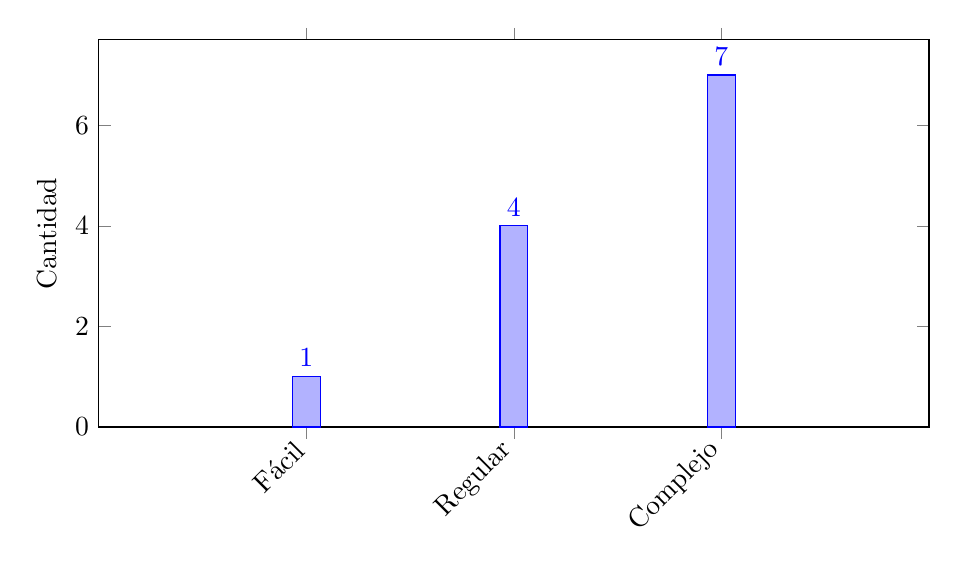
\begin{tikzpicture}
									\begin{axis}[
										ybar,
										width=\textwidth,
										height=6.5cm,
										symbolic x coords={Fácil, Regular, Complejo},
										xtick=data,
										ylabel={Cantidad},
										ymin=0,
										nodes near coords,
										enlarge x limits=0.5,
										x tick label style={rotate=45, anchor=east}
										]
										\addplot coordinates {(Fácil, 1) (Regular, 4) (Complejo, 7)};
									\end{axis}
								\end{tikzpicture}
								\subcaption{Facilidad del proceso de monitorización.}
								\label{fig:monitoring-process}
							\end{minipage}
							\vspace{5mm}
							\begin{minipage}{0.45\textwidth}
								\centering
								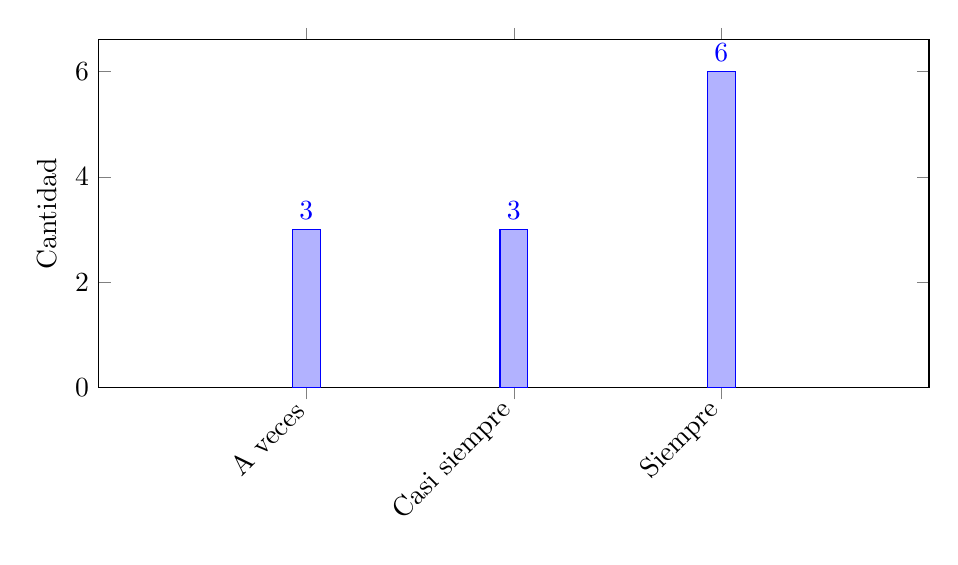
\begin{tikzpicture}
									\begin{axis}[
										ybar,
										width=\textwidth,
										height=6cm,
										symbolic x coords={A veces, Casi siempre, Siempre},
										xtick=data,
										ylabel={Cantidad},
										ymin=0,
										nodes near coords,
										enlarge x limits=0.5,
										x tick label style={rotate=45, anchor=east}
										]
										\addplot coordinates {(A veces, 3) (Casi siempre, 3) (Siempre, 6)};
									\end{axis}
								\end{tikzpicture}
								\subcaption{Frecuencia de monitorización.}
								\label{fig:monitoring-frequency}
							\end{minipage}
							\begin{minipage}{0.45\textwidth}
								\centering
								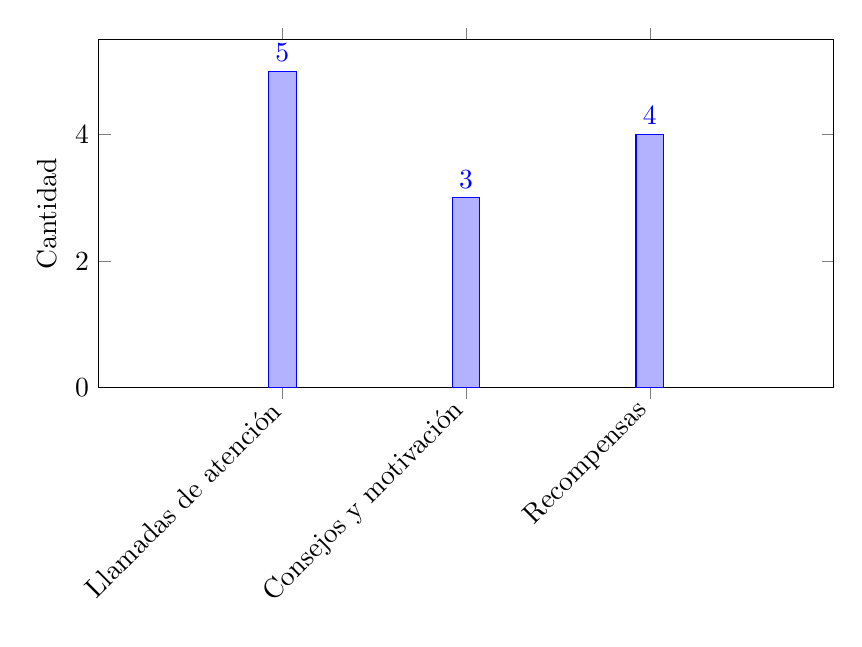
\begin{tikzpicture}
									\begin{axis}[
										ybar,
										height=6cm,
										width=0.9\textwidth,
										symbolic x coords={Llamadas de atención, Consejos y motivación, Recompensas},
										xtick=data,
										ylabel={Cantidad},
										ymin=0,
										nodes near coords,
										enlarge x limits=0.5,
										x tick label style={rotate=45, anchor=east}
										]
										\addplot coordinates {(Llamadas de atención, 5) (Consejos y motivación, 3) (Recompensas, 4)};
									\end{axis}
								\end{tikzpicture}
								\subcaption{Estrategias para lograr la concentración.}
								\label{fig:concentration-strategies}
							\end{minipage}
							\caption{Resultados de preguntas realizadas a los padres sobre el proceso de monitorización de sus hijos de primaria mientras hacen sus tareas.}
							\label{fig:previous-questions}
						\end{figure}
					
					\paragraph{\textbf{Tareas para los Usuarios Participantes:}}
						Las tareas que los tutores realizaron durante la evaluación fueron las siguientes:
					
						\begin{enumerate}
							\item Conectar el dispositivo Torddis a la fuente de alimentación y colocarlo en el escritorio donde el niño se sentará para realizar una tarea.
							\item Crear una cuenta de usuario tutor en la aplicación móvil.
							\item Iniciar sesión en la aplicación móvil.
							\item Registrar al niño que será monitoreado.
							\item Registrar el dispositivo Torddis en la aplicación móvil utilizando la dirección IP proporcionada en una etiqueta adherida al dispositivo.
							\item Realizar el entrenamiento facial para el niño registrado.
							\item Activar y/o desactivar los objetos que se monitorizarán en la sección correspondiente de la aplicación móvil.
							\item Asignar una tarea al niño mientras es monitoreado por el dispositivo Torddis: colorear un mandala.
							\item Activar el reconocimiento de cada parámetro de distracción en la sección de monitorización de la aplicación móvil.
							\item Dejar al niño solo, sin la presencia de un adulto, durante 6 minutos.
							\item Activar y/o desactivar la transmisión de video desde el dispositivo Torddis.
							\item Navegar por el historial de los parámetros de distracción monitoreados en el niño.
							\item Visualizar un informe con gráficos que representan los parámetros de distracción detectados para el niño monitoreado.
						\end{enumerate}
					
					\paragraph{\textbf{Resultados del Cuestionario System Usability Scale:}}
						Los resultados analizados en esta sección corresponden a las respuestas del cuestionario SUS (ver Apéndice \ref{Appendix:LikertScale}) proporcionado a los 12 tutores. Después de tabular los datos obtenidos, la Figura \ref{fig:sus-questionnaire} muestra que la media de los datos recopilados es 81.46\% con una desviación estándar de 11.65. Según los adjetivos (Peor imaginable, Pobre, OK, Bueno, Excelente, Mejor imaginable) propuestos por \cite{Bangor2008AnEmpirical} para evaluar cualitativamente la usabilidad de un sistema basado en la media alcanzada, es evidente que Torddis tiene un nivel de usabilidad "Bueno" según los tutores evaluados.
					
						\begin{figure}[hbt!]
							\centering
							\begin{tikzpicture}
								\begin{axis}[
									scatter/classes={
										a={mark=*,blue}
									},
									width=12cm,
									height=8cm,
									xlabel={Participante},
									ylabel={Evaluación},
									ymin=40, ymax=100,
									xmin=0, xmax=13,
									xtick={1,2,3,4,5,6,7,8,9,10,11,12},
									xticklabels={1,2,3,4,5,6,7,8,9,10,11,12},
									ytick={40,60,80,100},
									nodes near coords,
									every node near coord/.append style={font=\footnotesize, /pgf/number format/fixed},
									legend style={at={(0.5,-0.15)}, anchor=north, legend columns=-1},
									enlarge x limits=0.05,
									]
									\addplot[
									scatter,
									only marks,
									scatter src=explicit symbolic,
									visualization depends on=\thisrow{Evaluation} \as \label
									] table[meta=class,x=Participant,y=Evaluation] {
										Participant Evaluation class
										1 90.00 90.00
										2 95.00 95.00
										3 72.50 72.50
										4 60.00 60.00
										5 85.00 85.00
										6 67.50 67.50
										7 92.50 92.50
										8 67.50 67.50
										9 82.50 82.50
										10 85.00 85.00
										11 92.50 92.50
										12 87.50 87.50
									};
									
									% Línea de promedio
									\addplot [
									color=orange,
									thick,
									mark=none
									] coordinates {(0,\average) (13,\average)};
									
									% Línea de desviación estándar superior
									\addplot [
									color=orange,
									thick,
									dashed,
									mark=none
									] coordinates {(0,\upperlimit) (13,\upperlimit)};
									
									% Línea de desviación estándar inferior
									\addplot [
									color=orange,
									thick,
									dashed,
									mark=none
									] coordinates {(0,\lowerlimit) (13,\lowerlimit)};
									
									\legend{Participante, Promedio SUS, Desv. Estándar}
								\end{axis}
							\end{tikzpicture}
							\caption{Datos del cuestionario SUS por tutor con evaluación promedio y desviación estándar.}
							\label{fig:sus-questionnaire}
						\end{figure}
						
					\paragraph{\textbf{Resultados del Cuestionario de Preguntas Abiertas:}}
						Al final del cuestionario SUS, los tutores respondieron 8 preguntas abiertas (ver Apéndice \ref{Appendix:OpenQuestions}) para proporcionar sus opiniones personales.
					
						La primera pregunta fue "¿Cuál es su opinión general sobre el sistema?", a la que algunos tutores respondieron que apoya la concentración de los estudiantes, y otros dijeron que tiene un diseño agradable. Los resultados se muestran en la Figura \ref{fig:AboutTorddis}. La segunda pregunta abierta que respondieron los tutores fue "¿Le gustaron los sonidos y/o luces que utiliza Torddis?". La mayoría de los tutores presentaron una opinión favorable a esta pregunta, ya que creen que las alertas luminosas ayudan a mantener al estudiante despierto y están satisfechos con las alarmas sonoras (ver Figura \ref{fig:SoundAndLigth}).
					
						\begin{figure}[hbt!]
							\centering
							\begin{minipage}{0.45\textwidth}
								\centering
								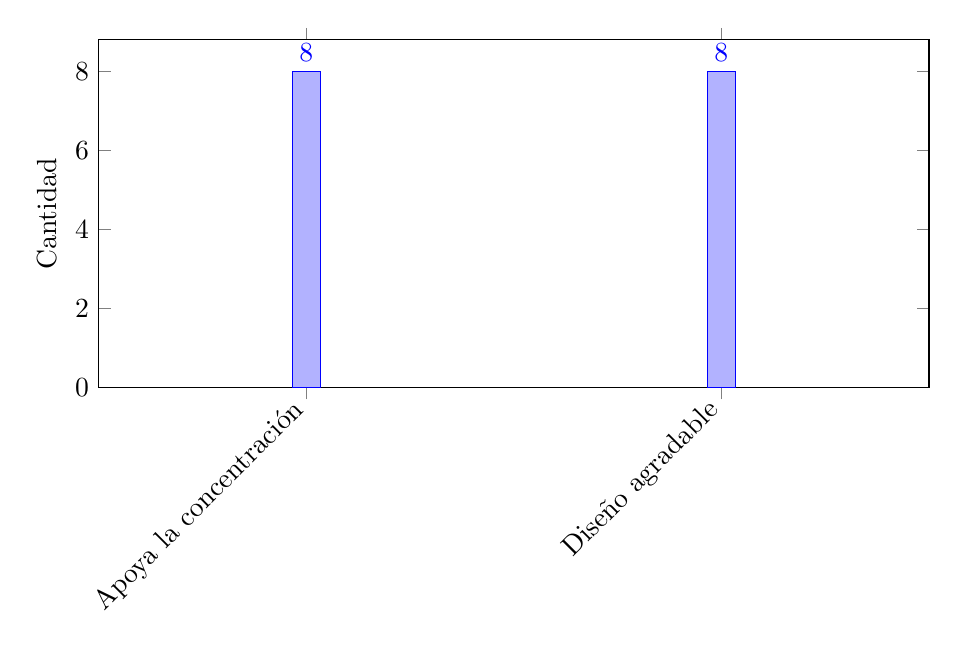
\begin{tikzpicture}
									\begin{axis}[
										ybar,
										width=\textwidth,
										height=6cm,
										symbolic x coords={Apoya la concentración, Diseño agradable},
										xtick=data,
										ylabel={Cantidad},
										ymin=0,
										nodes near coords,
										enlarge x limits=0.5,
										x tick label style={rotate=45, anchor=east}
										]
										\addplot coordinates {(Apoya la concentración, 8) (Diseño agradable, 8)};
									\end{axis}
								\end{tikzpicture}
								\subcaption{Opinión general sobre el sistema Torddis.}
								\label{fig:AboutTorddis}
							\end{minipage}
							\vspace{5mm}
							\begin{minipage}{0.45\textwidth}
								\centering
								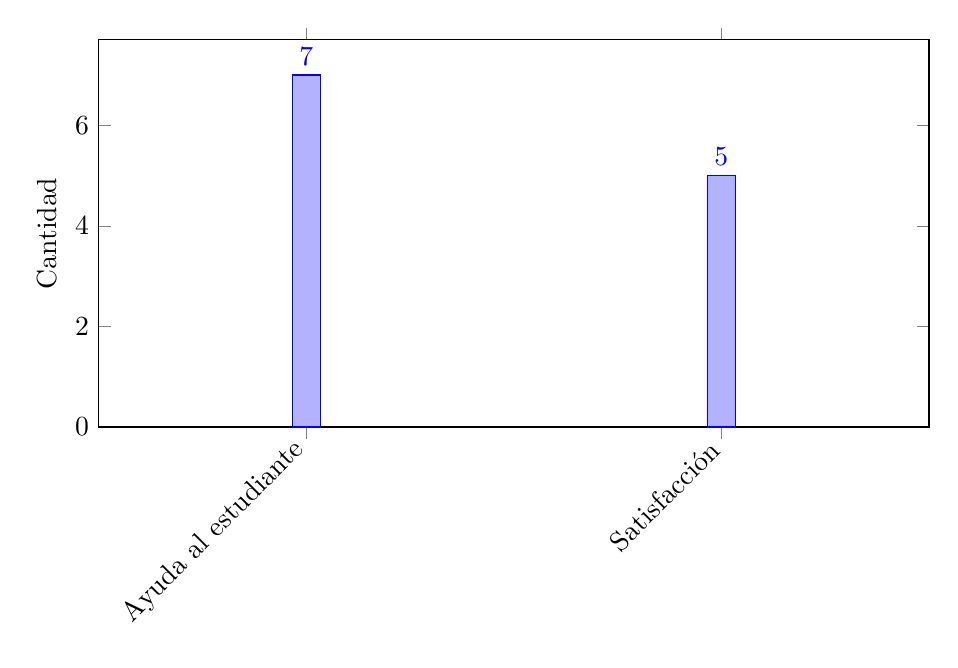
\begin{tikzpicture}
									\begin{axis}[
										ybar,
										width=\textwidth,
										height=6.5cm,
										symbolic x coords={Ayuda al estudiante, Satisfacción},
										xtick=data,
										ylabel={Cantidad},
										ymin=0,
										nodes near coords,
										enlarge x limits=0.5,
										x tick label style={rotate=45, anchor=east}
										]
										\addplot coordinates {(Ayuda al estudiante, 7) (Satisfacción, 5)};
									\end{axis}
								\end{tikzpicture}
								\subcaption{Alertas sonoras y luminosas del sistema.}
								\label{fig:SoundAndLigth}
							\end{minipage}
							\begin{minipage}{0.45\textwidth}
								\centering
								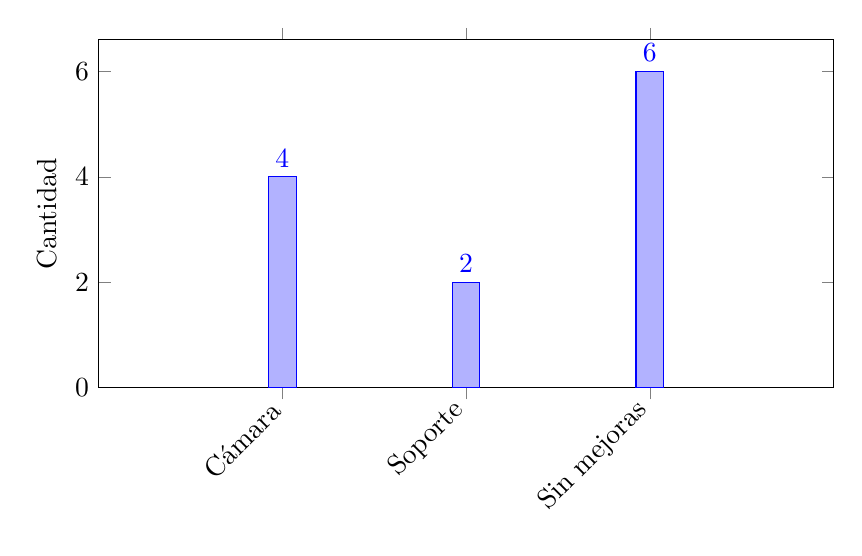
\begin{tikzpicture}
									\begin{axis}[
										ybar,
										height=6cm,
										width=0.9\textwidth,
										symbolic x coords={Cámara, Soporte, Sin mejoras},
										xtick=data,
										ylabel={Cantidad},
										ymin=0,
										nodes near coords,
										enlarge x limits=0.5,
										x tick label style={rotate=45, anchor=east}
										]
										\addplot coordinates {(Cámara, 4) (Soporte, 2) (Sin mejoras, 6)};
									\end{axis}
								\end{tikzpicture}
								\subcaption{Sugerencias para mejorar el sistema.}
								\label{fig:Improvements}
							\end{minipage}
							\begin{minipage}{0.45\textwidth}
								\centering
								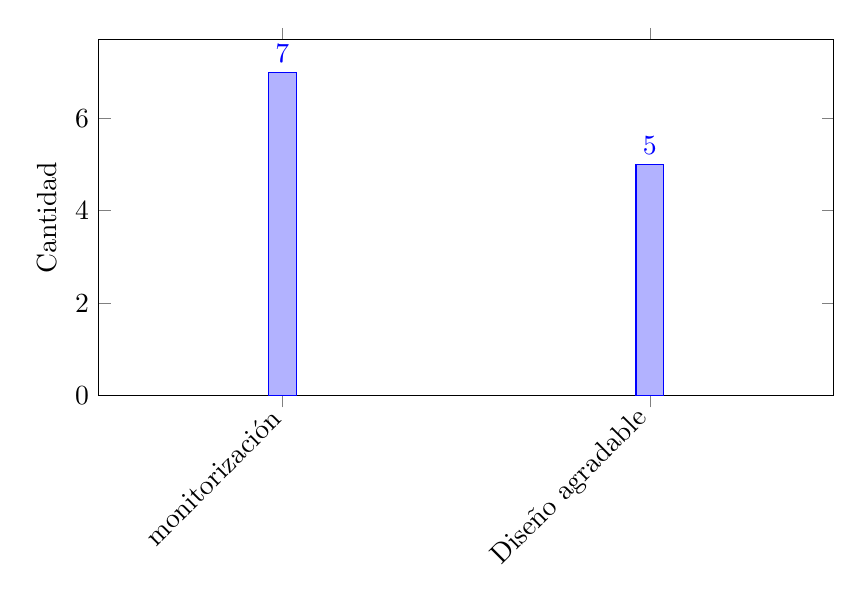
\begin{tikzpicture}
									\begin{axis}[
										ybar,
										height=6.1cm,
										width=0.9\textwidth,
										symbolic x coords={monitorización, Diseño agradable},
										xtick=data,
										ylabel={Cantidad},
										ymin=0,
										nodes near coords,
										enlarge x limits=0.5,
										x tick label style={rotate=45, anchor=east}
										]
										\addplot coordinates {(monitorización, 7) (Diseño agradable, 5)};
									\end{axis}
								\end{tikzpicture}
								\subcaption{Razones para recomendar el sistema.}
								\label{fig:ReasonsRecomend}
							\end{minipage}
							\caption{Resultados de preguntas realizadas a los padres sobre el proceso de monitorización de sus hijos de primaria usando Torddis mientras hacen sus tareas.}
							\label{fig:AnswerOfOpenQuestion}
						\end{figure}
						
						En las preguntas 3 ("¿Le gusta el diseño de la aplicación móvil Torddis? ¿Por qué?"), 4 ("¿Es adecuada la forma en que se visualizan los datos de monitorización de distracción de su hijo en la aplicación móvil Torddis? ¿Por qué?"), 5 ("¿Cree que este sistema ayudaría a mejorar la concentración de su hijo y mantenerlo informado mientras realiza sus tareas escolares? ¿Por qué?"), y 7 ("¿Estaría dispuesto a seguir usando el sistema Torddis?"), todos los tutores expresaron comentarios positivos. Manifestaron que les agrada el diseño de las vistas de la aplicación móvil, destacaron la organización de los datos históricos y los gráficos de informes, confirmaron que el sistema prototipo apoya eficazmente la concentración de los niños manteniéndolos informados cuando el niño se distrae, e indicaron su disposición a continuar usando el sistema Torddis.
						
						La pregunta 6 tenía como objetivo recopilar información sobre las mejoras que se podrían hacer a Torddis. Los comentarios obtenidos incluyen el uso de una cámara de mayor calidad y la mejora del soporte en el que se monta la cámara. Sin embargo, un alto porcentaje de usuarios mencionó que el dispositivo no necesita más mejoras. Estos resultados se muestran en la Figura \ref{fig:Improvements}. Por su parte, la pregunta 8 recopiló las razones por las que los evaluadores de Torddis recomendarían el uso de este sistema para la monitorización de estudiantes durante sus actividades escolares. La Figura \ref{fig:ReasonsRecomend} muestra las razones mencionadas por los tutores, incluyendo que les ayuda en la monitorización de sus estudiantes y su diseño agradable.
						
				\subsubsection*{Análisis de Reconocimiento}
					Esta subsección presenta los resultados de 14 pruebas realizadas utilizando el sistema Torddis, en las cuales se evaluaron cuatro tareas diferentes de reconocimiento: personas, expresiones faciales, presencia de sueño y objetos distractores. Cada prueba midió el tiempo en segundos que tomó reconocer el elemento correspondiente y registró si el reconocimiento fue exitoso o no. La Tabla \ref{tab:combined-recognition} muestra los datos recopilados para este análisis.
				
					\begin{table}[hbt!]
						\centering
						\caption{Resultados agregados de reconocimiento.}
						\label{tab:combined-recognition}
						\begin{tabularx}{\textwidth}{c >{\centering\arraybackslash}X c >{\centering\arraybackslash}X c >{\centering\arraybackslash}X c >{\centering\arraybackslash}X c}
							\toprule
							\textbf{No.} & \multicolumn{2}{c}{\textbf{Personas}} & \multicolumn{2}{c}{\textbf{Expresiones Faciales}} & \multicolumn{2}{c}{\textbf{Presencia de Sueño}} & \multicolumn{2}{c}{\textbf{Objetos Distractores}}\\
							\cline{2-9}
							& \textbf{Latencia} & \textbf{Logrado?} & \textbf{Latencia} & \textbf{Logrado?} & \textbf{Latencia} & \textbf{Logrado?} & \textbf{Latencia} & \textbf{Logrado?} \\
							\midrule
							1 & 0.57 & Sí & 1.50 & Sí & 5.10 & Sí & 0.00 & \textbf{No} \\
							2 & 0.60 & Sí & 1.20 & Sí & 3.50 & Sí & 1.68 & Sí \\
							3 & 0.00 & \textbf{No} & 0.70 & Sí & 0.00 & \textbf{No} & 0.00 & No \\
							4 & 0.78 & Sí & 1.30 & Sí & 3.68 & Sí & 1.79 & Sí \\
							5 & 1.02 & Sí & 0.78 & Sí & 2.24 & Sí & 0.00 & \textbf{No} \\
							6 & 0.88 & Sí & 1.01 & \textbf{No} & 2.63 & Sí & 1.98 & Sí \\
							7 & 0.53 & Sí & 1.23 & Sí & 0.00 & \textbf{No} & 1.73 & Sí \\
							8 & 1.20 & Sí & 0.97 & Sí & 2.03 & Sí & 2.05 & Sí \\
							9 & 0.76 & Sí & 1.05 & Sí & 4.09 & Sí & 1.77 & Sí \\
							10 & 1.20 & Sí & 0.70 & Sí & 3.36 & Sí & 1.91 & Sí \\
							11 & 0.69 & Sí & 1.99 & Sí & 4.69 & Sí & 4.27 & Sí \\
							12 & 0.82 & Sí & 1.83 & Sí & 3.29 & Sí & 2.69 & Sí \\
							13 & 0.93 & Sí & 1.68 & Sí & 3.14 & Sí & 2.81 & Sí \\
							14 & 0.58 & Sí & 1.76 & Sí & 3.45 & Sí & 2.94 & Sí \\
							\bottomrule
						\end{tabularx}
					\end{table}
					
					\paragraph{Tiempo total de reconocimiento: }
						\begin{itemize}
							\item \textbf{Tiempo total de reconocimiento en segundos para todas las pruebas}: 
							\begin{itemize}
								\item Personas: 10.56 segundos
								\item Expresiones Faciales: 17.70 segundos
								\item Sueño: 41.20 segundos
								\item Objetos Distractores: 25.62 segundos
							\end{itemize}
							\item \textbf{Número de reconocimientos exitosos}:
							\begin{itemize}
								\item Personas: 13
								\item Expresiones Faciales: 13
								\item Sueño: 12
								\item Objetos Distractores: 11
							\end{itemize}
							\item \textbf{Número de fallos en el reconocimiento}:
							\begin{itemize}
								\item Personas: 1
								\item Expresiones Faciales: 1
								\item Sueño: 2
								\item Objetos Distractores: 3
							\end{itemize}
						\end{itemize}
						
					\paragraph{Tiempo Promedio de Reconocimiento: }
						El tiempo promedio para los reconocimientos exitosos se calculó para cada tarea de reconocimiento:
						
						\begin{itemize}
							\item \textbf{Personas}: \(\frac{10.56 \text{ segundos}}{13} \approx 0.81 \text{ segundos}\)
							\item \textbf{Expresiones Faciales}: \(\frac{17.70 \text{ segundos}}{13} \approx 1.36 \text{ segundos}\)
							\item \textbf{Sueño}: \(\frac{41.20 \text{ segundos}}{12} \approx 3.43 \text{ segundos}\)
							\item \textbf{Objetos Distractores}: \(\frac{25.62 \text{ segundos}}{11} \approx 2.33 \text{ segundos}\)
						\end{itemize}
					
					\paragraph{Tasa de Reconocimiento: }
						La tasa de reconocimiento se determinó para cada tarea como el porcentaje de reconocimientos exitosos sobre el total de pruebas:
					
						\begin{itemize}
							\item \textbf{Personas}: \(92.86\%\)
							\item \textbf{Expresiones Faciales}: \(92.86\%\)
							\item \textbf{Sueño}: \(85.71\%\)
							\item \textbf{Objetos Distractores}: \(78.57\%\)
						\end{itemize}
						
					\paragraph{Tiempos Mínimos y Máximos de Reconocimiento: }
						Tiempos mínimos y máximos de reconocimiento observados en las pruebas para cada tarea:
						
						\begin{itemize}
							\item \textbf{Personas}:
							\begin{itemize}
								\item Tiempo mínimo: 0.00 segundos (Prueba 3)
								\item Tiempo máximo: 1.20 segundos (Pruebas 8 y 10)
							\end{itemize}
							\item \textbf{Expresiones Faciales}:
							\begin{itemize}
								\item Tiempo mínimo: 0.70 segundos (Pruebas 3 y 10)
								\item Tiempo máximo: 1.99 segundos (Prueba 11)
							\end{itemize}
							\item \textbf{Sueño}:
							\begin{itemize}
								\item Tiempo mínimo: 0.00 segundos (Pruebas 3 y 7)
								\item Tiempo máximo: 5.10 segundos (Prueba 1)
							\end{itemize}
							\item \textbf{Objetos Distractores}:
							\begin{itemize}
								\item Tiempo mínimo: 0.00 segundos (Pruebas 1, 3 y 5)
								\item Tiempo máximo: 4.27 segundos (Prueba 11)
							\end{itemize}
						\end{itemize}
					
					\paragraph{Distribución de los Tiempos de Reconocimiento:}
						Los tiempos de reconocimiento para cada tarea varían, lo que indica una variabilidad en la respuesta del sistema. La mayoría de los tiempos de reconocimiento están dentro de un rango razonable, lo que sugiere una respuesta rápida y efectiva del sistema en la mayoría de los casos.
					
			\subsubsection{Mantenimiento}
				Esta fase no fue ejecutada debido al corto tiempo de desarrollo para cada entregable, y además para la evaluación del proyecto. Sin embargo, el sistema debe ser mantenido bajo las indicaciones de prevención y de vida útil de cada uno de los componentes para funcionar correctamente. La Tabla \ref{tab:maintenance-tasks} describe algunas tareas de mantenimiento tentativas. En general, el mantenimiento del sistema se debe considerar hacerlo de manera trimestral y semestral, aunque su frecuencia puede variar dependiendo del entorno en el que se lo use.
			
				\begin{table}[h]
					\centering
					\caption{Definición de tareas de mantenimiento.}
					\label{tab:maintenance-tasks}
					\begin{tabularx}{\textwidth}{cXcc}
						\toprule
						\textbf{No.} & \textbf{Tareas de Mantenimiento} & \textbf{Trimestral} & \textbf{Semestral} \\
						\midrule
						1 & Limpieza interna del dispositivo. & * & \\
						2 & Verificar si los componentes del dispositivo tienen alguna imperfección o daño. & & * \\
						3 & Comprobar conexiones de cables, estado de los cables, conectores, etc. & & * \\
						4 & Probar el funcionamiento del zumbador y los LED. & * & \\
						5 & Probar el sistema informático (servidor de aplicaciones web, servicios web, aplicación móvil, dispositivo IoT). & & * \\
						\bottomrule
					\end{tabularx}
				\end{table}
				Los tiempos para el mantenimiento preventivo se consideran de acuerdo al componente con tiempo de vida útil. Así mismo¡, el mantenimiento correctivo por cada componente físico del sistema se debe realizar antes que la vida útil del componente llegue a su límite. La vida útil de cada uno de los componentes se muestra en la Tabla \ref{tab:ShelfLife}. El tiempo de vida útil de las resistencias se espera que sea significativamente mayor al del componente con la mayor durabilidad.
				
				\begin{table}[h]
					\centering
					\caption{Tiempo de vida útil de los componentes de hardware.}
					\label{tab:ShelfLife}
					\begin{tabularx}{\textwidth}{cXX}
						\toprule
						\textbf{Componente} & \textbf{Vida útil (años)} & Condiciones que reducen su vida útil\\
						\midrule
						Esp32CAM & 20 \citep{Espressif2022ESP32-CAM,Espressif2022ESP32Forum} & Exposición a temperaturas extremas, alta humedad, polvo o vibraciones mecánicas\\
						ESP8266 Node MCU & 20.83 \citep{Amri2018Improving} a 57 \citep{Ardumotica2023,Espressif2022ESP32Forum}. & Temperaturas extremas, niveles altos de humedad, polvo, picos de voltaje, ruido en la fuente, ciclo frecuentes de apagado y encendido, uso intenso de WiFi en máxima potencia, actualizaciones de firmware.\\
						Buzzer Pasivo & 3 \citep{HuawhaElectronics} & Voltaje excesivo, sobrecorriente, temperaturas extremas, vibraciones o impactos mecánicos, humedad o corrosión, operación continua prolongada. \\
						Leds & 3 \citep{Casamayor2015} - 14 \citep{Cary,GreenLighting2024} & Desgaste de componentes, condiciones de fabricación, \\
						Resistencias y otros & $\infty$ (se espera) & Tensiones altas \citep{Simon2017Evolution}. \\
						\bottomrule
					\end{tabularx}
				\end{table}
				La estimación de los años de vida útil de los componentes se ha fundamentado prioritariamente en referencias de documentos científicos. No obstante, en ausencia de fuentes académicas pertinentes, se han considerado las especificaciones proporcionadas por fabricantes y distribuidores, complementadas con información obtenida de foros especializados en ciertos casos.
				
		\subsection{Análisis estadístico del estudio}
				\subsubsection{Estadísticas Descriptivas}
				En esta sección de Resultados y Discusión, se presentan y analizan las estadísticas descriptivas obtenidas de los datos recolectados. Estas estadísticas desempeñan un papel crucial en el entendimiento del comportamiento de las variables evaluadas y su impacto en la aceptación y efectividad del sistema.
				
				la tabla \ref{table:DescriptiveStatistics} muestra las métricas de tendencia central, como la media y la mediana, permiten identificar patrones generales en las respuestas de los tutores y estudiantes. Por ejemplo, el tiempo promedio dedicado por los tutores a la supervisión de tareas escolares de manera diaria es de 2 horas, lo que indica una participación activa pero limitada debido a restricciones de tiempo. Las respuestas a las afirmaciones relacionadas con la percepción y uso del dispositivo (1 a 7) reflejan valores medios consistentemente altos (entre 3.58 y 4.42), lo que sugiere una aceptación generalizada del sistema.
				
				\begin{table}[h!]
					\centering
					\caption{Estadísticas Descriptivas}
					\begin{tabularx}{0.85\textwidth}{Xcccccccc}
						\toprule
						\textbf{Estadística} & \textbf{Horas de Supervisión} & \textbf{(1)} & \textbf{(2)} & \textbf{(3)} & \textbf{(4)} & \textbf{(5)} & \textbf{(6)} & \textbf{(7)} \\
						\midrule
						Media & 2.00 & 4.42 & 4.42 & 2.67 & 3.58 & 4.00 & 4.42 & 4.42 \\
						Mediana & 2.00 & 5.00 & 4.00 & 3.00 & 4.00 & 4.00 & 5.00 & 5.00 \\
						Desviación estándar & 0.69 & 0.90 & 0.67 & 0.98 & 0.90 & 0.85 & 0.79 & 0.79 \\
						Mínimo & 1.00 & 3.00 & 3.00 & 1.00 & 2.00 & 3.00 & 3.00 & 3.00 \\
						Máximo & 3.00 & 5.00 & 5.00 & 4.00 & 5.00 & 5.00 & 5.00 & 5.00 \\
						\bottomrule
					\end{tabularx}
					\label{table:DescriptiveStatistics}
					\vspace{0.3em} % Espaciado entre la tabla y el pie
					\parbox{0.85\textwidth}{\footnotesize \centering
						(1): Afirmación (1), Afirmación (2),..., Afirmación (7).\\
						\textit{Horas de supervisión} representa el tiempo diario que los tutores dedican a la supervisión de sus hijos en cuánto a la realización de tareas escolares. Las \textit{Afirmaciones de la (1) a la (7)} corresponden a los ítems evaluados en la escala de Likert relacionada con la efectividad del prototipo (ver anexo \ref{Appendix:Effectivity}).
					}
				\end{table}
				
				Por otro lado, los indicadores de dispersión, como la desviación estándar, ofrecen información sobre la variabilidad de las respuestas. La desviación estándar de las afirmaciones (0.67 a 0.98) indica que las percepciones de los participantes fueron relativamente homogéneas, lo que refuerza la consistencia en la experiencia de uso del dispositivo. Sin embargo, la mayor variabilidad en la afirmación (3) sugiere que algunos estudiantes pudieron percibir más intrusividad en el dispositivo, lo que podría requerir ajustes de diseño.
				
				Asimismo, los valores mínimos y máximos revelan las posibles diferencias en la experiencia de los participantes, destacando áreas que podrían mejorarse. Por ejemplo, algunos tutores dedicaron solo 1 hora a la supervisión, mientras que otros alcanzaron las 3 horas, lo que podría influir en las respuestas relacionadas con la efectividad del sistema.
				
				Estos resultados permiten identificar no solo el nivel de aceptación general del sistema, sino también las áreas que podrían beneficiarse de intervenciones específicas. En conjunto, las estadísticas descriptivas proporcionan un marco para validar el diseño del dispositivo y fundamentar la discusión sobre su potencial pedagógico y práctico.
				
				\subsubsection{Análisis de la Normalidad de los Datos}
					Para evaluar si las variables continuas, como la edad del tutor, horas de supervisión y edad del estudiante, siguen una distribución normal se realizó la prueba de Shapiro-Wilk. Los resultados se muestra en la Tabla \ref{table:Shaphiro-Wilk}.
					
					\begin{table}[h!]
						\centering
						\caption{Resultados del análisis de normalidad mediante la prueba de Shapiro-Wilk}
						\begin{tabularx}{0.75\textwidth}{Xccc}
							\toprule
							\textbf{Variable} & \textbf{Estadístico} &  \textbf{p-valor} & \textbf{Distribución Normal} \\
							\midrule
							Edad del tutor & 0.912 & 0.228 & \(\checkmark\) \\
							Localización de la vivienda & 0.640 & 0.000 & \(\times\) \\
							Horas de supervisión & 0.809 & 0.012 & \(\times\) \\
							Edad del estudiante & 0.903 & 0.174 & \(\checkmark\) \\
							Afirmación (1) & 0.729 & 0.002 & \(\times\) \\
							Afirmación (2) & 0.784 & 0.002 & \(\times\) \\
							Afirmación (3) & 0.863 & 0.053 & \(\checkmark\) \\
							Afirmación (4) & 0.867 & 0.060 & \(\checkmark\) \\
							Afirmación (5) & 0.828 & 0.020 & \(\times\) \\
							Afirmación (6) & 0.828 & 0.020 & \(\times\) \\
							Afirmación (7) & 0.729 & 0.002 & \(\times\) \\
							\bottomrule
						\end{tabularx}
						\label{table:Shaphiro-Wilk}
						\vspace{0.3em} % Espaciado entre la tabla y el pie
						\parbox{0.75\textwidth}{\footnotesize \centering
							\(\times\): No sigue una distribución normal. \(\checkmark\): Sigue una distribución normal.\\
							La variable "\textit{localización de la vivienda}", representa si la vivienda está en el sector rural o urbano. La columna \textit{Estadístico} muestra los valores de los coeficientes obtenidos mediante la prueba de Shapiro-Wilk. El \textit{p-valor} representa el nivel de significancia de la prueba.
						}
					\end{table}
					
					El \textit{p-valor} de la Tabla \ref{table:Shaphiro-Wilk}, indica si se acepta o rechaza la hipótesis nula, es decir, si las variables siguen o no una distribución normal. En la columna \textit{Distribución Normal}, muestran la conclusión de las pruebas de hipótesis (H0 : La variable sigue una distribución normal. H1: la variable no sigue una distribución normal.)
					
					Los resultados de la prueba de Shapiro-Wilk indicaron que algunas variables seguían una distribución normal, mientras que otras no lo hacían. Para garantizar la validez de los análisis posteriores, se seleccionaron pruebas estadísticas adecuadas en función de estos resultados.
					
					\paragraph{\textbf{Variables con distribución normal:}}
					Las variables "Edad del tutor", "Edad del estudiante", "Afirmación \textit{(3) Su tutorado tomó desapercibida la presencia del dispositivo}" y "Afirmación (4) \textit{Utilizó el dispositivo todo el tiempo efectivo dedicado para hacer las tareas}" mostraron un p-valor mayor a 0.05, lo que permitió emplear pruebas paramétricas. Se utilizaron pruebas de correlación de Pearson y análisis de varianza (ANOVA) para explorar las relaciones y diferencias significativas entre estas variables y los factores correspondientes.
					
					\paragraph*{Coeficientes de Correlación de Pearson:}
					En la Tabla \ref{table:Pearson-Correlation} se presentan los resultados de la relación entre la afirmación (5) y las variables con distribución normal, utilizando los coeficientes de correlación de Pearson.
					
					\begin{table}[h!]
						\centering
						\caption{Correlaciones entre las variables con distribución normal}
						\begin{tabularx}{0.75\textwidth}{Xccc}
							\toprule
							\textbf{Variable} & \textbf{Correlación con Afirmación (5)} &  \textbf{p-valor} & \textbf{Tipo de relación} \\
							\midrule
							Edad del tutor & 0.272 & 0.392 & \(\times\) \\ % Sin relación significativa
							Edad del estudiante & -0.141 & 0.663 & \(\times\) \\ % Sin relación significativa
							Afirmación (3) & 0.750 & 0.005 & \(\bigtriangleup\) \\ % Relación moderada
							Afirmación (4) & 0.816 & 0.001 & \(\checkmark\) \\ % Relación fuerte
							\bottomrule
						\end{tabularx}
						\label{table:Pearson-Correlation}
						\vspace{0.3em} % Espaciado entre la tabla y el pie
						\parbox{0.75\textwidth}{\footnotesize \centering
							\(\times\): Sin relación significativa. \(\bigtriangleup\): Relación moderada. \(\checkmark\): Relación fuerte
						}
					\end{table}
					
					El análisis de \textit{\textbf{correlaciones de Pearson}} permitió identificar las relaciones entre las variables con distribución normal y la afirmación (5), "\textit{Después de dejar de usar el dispositivo, su tutorado mejoró el nivel de autorregulación y concentración en la realización de tareas}". Las correlaciones observadas fueron estadísticamente significativas en varios casos, lo que destaca patrones importantes sobre el impacto del dispositivo.
					
					En primer lugar, las variables de las afirmaciones (3) \textit{"Su tutorado tomó desapercibida la presencia del dispositivo"} y (4) "\textit{Utilizó el dispositivo todo el tiempo efectivo dedicado para hacer las tareas}" presentaron correlaciones positivas fuertes con la \textit{afirmación (5)}, con valores de \textbf{0.750} y \textbf{0.816} respectivamente. Esto sugiere que el diseño no intrusivo del dispositivo (afirmación 3) y su uso efectivo durante el tiempo dedicado a las tareas (afirmación 4) son factores clave que contribuyen a la mejora percibida en la autorregulación. La fortaleza de estas correlaciones resalta la importancia de la usabilidad y la funcionalidad del dispositivo en la experiencia del usuario.
					
					La edad suele percibirse como un indicador de mayor responsabilidad \citep{Moss2018Why}. Sin embargo, en este estudio, las variables "\textit{Edad del tutor}" y "\textit{Edad del estudiante}" mostraron correlaciones débiles y no significativas, con valores de \textbf{0.272} y \textbf{-0.141}, respectivamente. Estos hallazgos sugieren que la efectividad percibida del dispositivo no está influenciada ni por la edad de los tutores ni por la de los estudiantes. Este resultado resalta la versatilidad del sistema, demostrando su aplicabilidad en diversos grupos demográficos sin verse limitado por factores relacionados con la edad.
					
					Finalmente, los resultados obtenidos subrayan que las características directamente relacionadas con el uso del dispositivo, como su diseño y efectividad operativa, tienen un mayor impacto en la mejora de la autorregulación que los factores demográficos. Esto proporciona evidencia sólida para el diseño centrado en el usuario como una estrategia clave en el desarrollo de sistemas educativos basados en tecnología.
					
					\paragraph*{Análisis ANOVA:}
					
					\begin{table}[h!]
						\centering
						\caption{Resultados del Análisis ANOVA}
						\begin{tabularx}{0.75\textwidth}{Xcrrrrc}
							\toprule
							\textbf{Variable} & \textbf{df} &  \textbf{sum\_sq} & \textbf{mean\_sq} & \textbf{F} & \textbf{PR(>F)} & \textbf{Conclusión}\\
							\midrule
							Edad del tutor & 1 & 0.445 & 0.445 & 2.984 & 0.128 & \(\times\)  \\ %No hay diferencias significativas.
							Edad del estudiante & 1 & 0.006 & 0.006 & 0.041 & 0.846 & \textit{NS}\\ % Sin efecto significativo.\\ 
							Afirmación (3) & 1 & 3.031 & 3.031 & 20.306 & 0.003 & \(\bigstar\) \\ % Relación altamente significativa.
							Afirmación (4) & 1 & 1.473 & 1.473 & 9.868 & 0.016 & \(\checkmark\) \\ %Relación significativa.
							Residual & 7 & 1.045 & 0.149 & NaN & NaN & \faExclamationTriangle \\ %Contribución acumulada de la variabilidad no explicada.
							\bottomrule
						\end{tabularx}
						\label{table:ANOVA-Results}
						\vspace{0.3em} % Espaciado entre la tabla y el pie
						\parbox{0.75\textwidth}{\footnotesize 
							\(\times\): No hay diferencias significativas. \textit{NS}: Sin efecto significativo. \(\checkmark\): Relación significativa. \(\bigstar\): Relación altamente significativa. \faExclamationTriangle: Contribución acumulada de la variabilidad no explicada: Modelo mejorable.
						}
					\end{table}
					
					El valor residual refleja la porción de variabilidad en los datos que no ha sido explicada por las variables consideradas en el modelo. Este valor indica que, aunque algunas variables, como las afirmaciones (3) y (4), muestran efectos significativos en la afirmación (5), existe una parte de la variabilidad que no puede atribuirse directamente a las variables incluidas.
					
					En este caso, el residual sugiere que hay factores adicionales, posiblemente no considerados en este modelo, que también influyen en la percepción de mejora en la autorregulación tras el uso del dispositivo. Estos factores podrían estar relacionados con características individuales de los tutores o estudiantes, el contexto específico de las pruebas, o incluso aspectos técnicos del dispositivo que no fueron directamente medidos.
					
					\paragraph{\textbf{Variables sin distribución normal:}}
					Para las variables "Horas de supervisión", "Afirmación \textit{(1) El dispositivo fue tomado por su tutorado como algo atractivo}", "Afirmación \textit{(2) La aplicación móvil mostró correctamente los eventos que sucedieron}", "Afirmación \textit{(6) Aunque es poco tiempo de utilización del dispositivo, mejoraría considerablemente el cumplimiento de tareas, por ende el nivel de aprovechamiento de los estudios de su tutorado.}" y "Afirmación \textit{(7) Está dispuesto a seguir utilizando el dispositivo}", cuyo p-valor fue menor a 0.05, se realizaron pruebas no paramétricas. En este caso, se aplicó el coeficiente de correlación de Spearman para evaluar las relaciones entre estas variables y se utilizó la prueba de Kruskal-Wallis para analizar diferencias entre grupos categóricos.
					
					\paragraph*{Coeficientes de Correlación de Spearman: }
					En la Tabla \ref{table:Spearman-Correlation} se muestran los resultados del coeficiente de Spearman.
						
					\begin{table}[h!]
						\centering
						\caption{Correlaciones entre las variables con distribución No normal}
						\begin{tabularx}{0.85\textwidth}{Xccc}
							\toprule
							\textbf{Variable} & \textbf{Correlación con Afirmación (5)} &  \textbf{p-valor} & \textbf{Tipo de relación} \\
							\midrule
							Tiempo de supervisión de tareas & 0.192 & 0.549 & \(\times\)  \\ % (Sin relación significativa) \\
							Afirmación (1) & 0.770 & 0.003 & \(\checkmark\) \\ %(Relación fuerte)
							Afirmación (2) & 0.551 & 0.063 & \(\bigtriangleup\)  \\ %(Relación moderada)
							Afirmación (6) & 1.000 & 0.000 & \(\bigstar\)  \\ %(Relación perfecta)
							Afirmación (7) & 0.770 & 0.003 & \(\checkmark\)  \\ %(Relación fuerte)
							\bottomrule
						\end{tabularx}
						\label{table:Spearman-Correlation}
						\vspace{0.3em} % Espaciado entre la tabla y el pie
						\parbox{0.75\textwidth}{\footnotesize 
							\(\times\): Sin relación significativa. \(\bigtriangleup\): Relación moderada. \(\bigstar\): Relación perfecta. \(\checkmark\): Relación fuerte.
						}
					\end{table}
					
					Los resultados del análisis de \textit{\textbf{correlación de Spearman}} proporcionaron información valiosa sobre las relaciones entre las variables con distribución no normal y la Afirmación (5).
					
					La Afirmación (1) mostró una correlación fuerte y significativa (\textbf{0.770}, \textit{p}=0.003), lo que indica que la percepción positiva inicial del dispositivo está altamente relacionada con la mejora percibida en la autorregulación del estudiante. Esto subraya la importancia del diseño atractivo y funcional del dispositivo como factor clave para fomentar el uso y obtener resultados positivos.
					
					Por otro lado, la Afirmación (2) presentó una correlación moderada pero no significativa (\textbf{0.551, p=0.063}). Aunque los resultados no permiten confirmar una relación estadísticamente significativa, la tendencia observada sugiere que la precisión en la detección de eventos puede contribuir a generar confianza en el sistema, lo que podría tener un impacto indirecto en la percepción de su efectividad.
					
					En el caso de la Afirmación (6), se observó una correlación perfecta (\textbf{1.00, p=0.000}). Esto refleja una dependencia completa entre esta variable y la mejora percibida en la autorregulación, lo cual puede interpretarse como una validación directa de la efectividad del dispositivo en contextos específicos.
					
					Finalmente, la Afirmación (7) mostró una correlación fuerte y significativa (\textbf{0.770, p=0.003}). Este resultado resalta la aceptación general del sistema entre los usuarios y su disposición a continuar utilizándolo, lo que puede ser un indicador de la sostenibilidad del dispositivo en el tiempo.
					
					\paragraph*{Prueba de Kruskal-Wallis para Determinar las Diferencias entre Grupos Categóricos: }
					Al aplicar la \textbf{\textit{prueba de Kruskal-Wallis}} se determinó la relación entre grupos categóricos con la Afirmación (5). Los resultados que se obtuvieron en la prueba de Kruskal-Wallis se muestran en la Tabla \ref{table:Kruskal-Wallis}.
					
					\begin{table}[h!]
						\centering
						\caption{Resultados de la Prueba de Kruskal-Wallis para Variables Categóricas}
						\begin{tabularx}{0.75\textwidth}{Xccc}
							\toprule
							\textbf{Variable} & \textbf{Estadístico} &  \textbf{p-valor} & \textbf{Conclusión} \\
							\midrule
							Localización de la residencia & 18.223 & 1.965 & \(\times\) \\ % No se encontraron diferencias significativas.
							Formación del tutor & 18.223 & 1.965 & \(\times\) \\ % No se encontraron diferencias significativas. \\
							Género del tutor & 18.374 & 1.814 &  \(\times\) \\ % No se encontraron diferencias significativas.
							\bottomrule
						\end{tabularx}
						\label{table:Kruskal-Wallis}
						\vspace{0.3em} % Espaciado entre la tabla y el pie
						\parbox{0.75\textwidth}{\footnotesize 
							\(\times\): No se encontraron diferencias significativas.
						}
					\end{table}
					
					Que no existan diferencias significativas en un análisis estadístico, como en este caso con la prueba de Kruskal-Wallis, significa que no se puede rechazar la hipótesis nula, que establece que las medianas de los grupos comparados son iguales. En otras palabras, los datos no proporcionan evidencia suficiente para afirmar que existe una diferencia real entre los grupos categóricos analizados en relación con la variable de interés, en este caso, la Afirmación (5).
						
	\section{Conclusiones}
	\label{seccion:Seis}
		El sistema prototipo Torddis aporta un avance significativo en el campo de la pedagogía tecnológica, combinando IoT e IA para abordar desafíos críticos en el aprendizaje autónomo \citep{DiPietro2025Meta}. A diferencia de propuestas previas, el sistema integra análisis de comportamiento en tiempo real con retroalimentación activa, destacando su contribución al desarrollo de teorías sobre autorregulación y aprendizaje personalizado en entornos domésticos. Las evaluaciones, que incluyen pruebas funcionales y cuestionarios de usabilidad, revelaron que el sistema cumple con los requisitos técnicos esperados y es altamente valorado por los usuarios finales, es decir, los tutores.
		
		El análisis de los datos demográficos y de monitorización indica que Torddis tiene un impacto significativo en la gestión de la distracción de los niños, proporcionando a los tutores una herramienta valiosa para mantener a los estudiantes enfocados en sus tareas. La alta puntuación en el cuestionario de usabilidad SUS refuerza la percepción de que el sistema es fácil de usar y efectivo en su propósito.
		
		El sistema de reconocimiento de personas de Torddis es eficiente, con una tasa de éxito del 92.86\% y un tiempo promedio de reconocimiento de aproximadamente 0.81 segundos, demostrando un sólido desempeño en condiciones de prueba. Del mismo modo, el sistema de reconocimiento de expresiones faciales muestra una tasa de éxito del 92.86\% con un tiempo promedio de reconocimiento de aproximadamente 1.36 segundos, destacando por sus tiempos de respuesta rápidos y su fiabilidad. El sistema de reconocimiento de la presencia de sueño es razonablemente eficiente, alcanzando una tasa de éxito del 85.71\% y un tiempo promedio de reconocimiento de aproximadamente 3.43 segundos, lo que indica un rendimiento adecuado.
		
		El sistema de reconocimiento de objetos distractores, con una tasa de éxito del 78.57\% y un tiempo promedio de reconocimiento de aproximadamente 2.33 segundos, funciona adecuadamente en condiciones de prueba.
		
		Además, los comentarios de las preguntas abiertas muestran un fuerte respaldo al diseño y funcionalidad del sistema, con valiosas sugerencias para futuros desarrollos. Los tutores destacaron la importancia de las alertas visuales y auditivas para mantener a los estudiantes alertas y la conveniencia de las opciones de configuración y monitorización del sistema.
		
		En conclusión, Torddis ha superado las expectativas en términos de funcionalidad y usabilidad, demostrando ser una solución viable y efectiva para mantener la concentración de los estudiantes en entornos de aprendizaje. El éxito de este proyecto subraya la importancia de la innovación tecnológica en la educación y sienta las bases para futuras mejoras y expansiones del sistema.
	
		(ANOVA) La presencia de un residual notable refuerza la idea de que, aunque el modelo es útil para identificar relaciones significativas, no agota todas las explicaciones posibles, lo que abre la puerta a investigaciones futuras para explorar otras variables que puedan complementar el análisis actual.
		
		En resumen, los resultados del análisis de Spearman destacan cómo factores como la percepción inicial del dispositivo, su precisión y su aceptación por parte de los usuarios influyen en la efectividad percibida. Este enfoque refuerza la importancia de integrar estos elementos en el diseño y evaluación de tecnologías educativas para garantizar su éxito en contextos diversos.
		
	\section*{Agradecimientos}
	
	Este trabajo de investigación ha sido financiado por la subvención PID2022-139297OB-I00, financiada por MICIU/AEI/10.13039/501100011033 y por el FEDER/UE.
	
	\printcredits
	
	\bibliographystyle{cas-model2-names}
	
	% Loading bibliography database
	\bibliography{torddisC&E-refs}
	
	\clearpage
	
	\appendix
	\section{Consentimiento Informado} \label{Appendix:InformedConsent}
	Estimado Participante,
	
	El propósito de este documento es proporcionarle la información necesaria para decidir si desea o no participar en el proyecto titulado "Sistema basado en Internet de las Cosas para monitorizar la distracción de niños durante sus actividades académicas en casa", realizado bajo la dirección del Profesor Gleiston Cicerón Guerrero Ulloa MDS.
	
	La participación implica el uso del sistema proporcionado, siguiendo las instrucciones de los investigadores. Se le pedirá que se siente en un lugar específico para utilizar una aplicación móvil. Mientras tanto, su hijo será monitoreado por un dispositivo inteligente llamado "Torddis" mientras realiza una tarea específica dirigida por los investigadores. El tiempo de participación es de aproximadamente 30 minutos, dependiendo de cada participante. Estas actividades se realizarán en una de las casas de los investigadores.
	
	La información obtenida a través de este estudio se mantendrá estrictamente confidencial y sus nombres no serán utilizados. Usted tiene el derecho de retirar el consentimiento para participar en cualquier momento. El estudio no implica ningún riesgo para usted, ni recibirá compensación alguna. Si tiene alguna pregunta sobre este proyecto, puede contactarnos en gguerrero@uteq.edu.ec.
	
	\vspace{0.5cm}
	\noindent\rule{3.65cm}{0.4pt} \hspace{1.1cm} \rule{4cm}{0.4pt} \hspace{1.1cm} \rule{4.2cm}{0.4pt}\\
	Carlos Almeida-Dueñas \hspace{2cm} John Plazarte-Suárez \hspace{2cm} Gleiston Guerrero-Ulloa
	
	Después de leer el procedimiento descrito anteriormente, de que los investigadores le expliquen el procedimiento y de responder a cualquier pregunta, el participante (firmante) da voluntariamente su consentimiento para participar en este estudio.
	
	\vspace{0.5cm}
	\noindent
	Participante: \_\_\_\_\_\_\_\_\_\_\_\_\_\_\_\_\_\_\_\_\_\_\_\_\_\_\_\_\_\_\_\_\_\_\_\_
	Firma: \_\_\_\_\_\_\_\_\_\_\_\_\_\_\_\_\_\_\_\_\_\_\_\_
	Fecha: \_\_\_\_\_\_\_\_\_\_
	
	\clearpage
	\section[\appendixname~\thesection]{Encuesta Demográfica} \label{Appendix:DemographicSurvey}
	\vspace{12pt}
	\noindent
	\textbf{1. Nombre Completo: \_\_\_\_\_\_\_\_\_\_\_\_\_\_\_\_\_\_\_\_\_\_\_\_\_\_\_\_\_\_\_\_\_\_\_\_\_\_\_\_\_\_\_\_\_}
	
	\vspace{12pt}
	\noindent
	\textbf{2. Edad: \_\_\_\_\_\_\_\_\_\_}
	
	\vspace{12pt}
	\noindent				
	\textbf{3. Nivel de Educación:}
	
	\begin{itemize}
		\item Sin educación ( )
		\item Primaria ( )
		\item Secundaria ( )
		\item Superior ( )
	\end{itemize}
	
	\noindent
	\textbf{4. Género:}
	
	\begin{itemize}
		\item Masculino ( )
		\item Femenino ( )
		\item Otro ( )
	\end{itemize}
	
	%\vspace{12pt.}
	\noindent
	\textbf{5. ¿Cómo ha sido su experiencia como padre en monitorizar las distracciones de su hijo mientras realiza sus tareas escolares?}
	
	\begin{itemize}
		\item Fácil ( )
		\item Regular ( )
		\item Compleja ( )
		\item Muy compleja ( )
	\end{itemize}
	
	%\vspace{12pt.}
	\noindent
	\textbf{6. ¿Con qué frecuencia monitoriza las actividades escolares de su hijo?}
	
	\begin{itemize}
		\item Nunca ( )
		\item A veces ( )
		\item Casi siempre ( )
		\item Siempre ( )
	\end{itemize}
	
	%\vspace{12pt.}
	\noindent
	\textbf{7. ¿Qué estrategias ha implementado para mejorar la concentración de su hijo durante sus tareas escolares?}
	
	\vspace{12pt}
	\noindent
	\rule{\textwidth}{1pt}
	
	\vspace{12pt}
	\noindent
	\rule{\textwidth}{1pt}
	
	\clearpage
	\section[\appendixname~\thesection]{Cuestionario SUS}
	\label{Appendix:SUSQuestionarie}
	
	
	\subsection[\appendixname~\thesection]{Cuestionario en Escala Likert}
	\label{Appendix:LikertScale}
	Las preguntas del cuestionario SUS usando la escala Likert se muestran en la Tabla \ref{tab:SUSQuestion}.
	
	\begin{table}[bt!]
		\caption{Cuestionario SUS \label{tab:SUSQuestion}}
		\centering
		\begin{tabular}{|p{10cm}|c|c|c|c|c|}
			\hline
			\textbf{Preguntas} & 1 & 2 & 3 & 4 & 5 \\
			\hline
			1. Me gustaría utilizar el sistema Torddis frecuentemente. & & & & & \\
			\hline
			2. Encontré el sistema innecesariamente complejo. & & & & & \\
			\hline
			3. Pensé que el sistema era fácil de usar. & & & & & \\
			\hline
			4. Necesitaría el apoyo de un técnico/profesor para usar el sistema. & & & & & \\
			\hline
			5. Encontré que las diversas funciones del sistema estaban bien integradas (constituían un todo). & & & & & \\
			\hline
			6. Pensé que había demasiadas inconsistencias en el sistema. & & & & & \\
			\hline
			7. Me imagino que la mayoría de las personas aprenderían a usar el sistema rápidamente. & & & & & \\
			\hline
			8. Encontré el sistema muy difícil de usar. & & & & & \\
			\hline
			9. Me sentí muy seguro/cómodo usando el sistema. & & & & & \\
			\hline
			10. Necesito aprender muchas cosas antes de poder usar el sistema. & & & & & \\
			\hline
		\end{tabular}
	\end{table}
	
	\subsection[\appendixname~\thesection]{Preguntas Abiertas del Cuestionario SUS}
	\label{Appendix:OpenQuestions}
	Las preguntas abiertas del cuestionario SUS se muestran en la Tabla \ref{tab:OpenQuestion}.
	\begin{table}[bt!]
		\centering
		\caption{Preguntas Abiertas del Cuestionario SUS \label{tab:OpenQuestion}}
		\begin{tabularx}{\textwidth}{c X }
			\toprule
			\textbf{No.} & \textbf{Pregunta} \\
			\midrule
			1 & En general, ¿cuál es su opinión sobre el sistema? \\
			2 & ¿Le gustaron los sonidos y/o luces que contiene el dispositivo Torddis? Por favor responda sí o no, y proporcione la razón. \\
			3 & ¿Le gustó el diseño de la pantalla de la aplicación móvil de Torddis? Por favor responda sí o no, y proporcione la razón. \\
			4 & ¿Le parece adecuada la forma en que se visualizan los datos de monitorización de distracción de su hijo en la aplicación móvil Torddis? Por favor responda sí o no, y proporcione sugerencias. \\
			5 & ¿Cree que este sistema ayudaría a mejorar la concentración de su hijo y a mantenerle informado cuando esté distraído? Por favor responda sí o no, y proporcione la razón. \\
			6 & ¿Cree que hay algo que debería mejorarse en el sistema Torddis (Dispositivo y Aplicación Móvil)? En caso afirmativo, ¿qué? \\
			7 & ¿Estaría dispuesto a continuar usando el sistema Torddis? Por favor responda sí o no, y proporcione la razón. \\
			8 & ¿Recomendaría este sistema a otras personas interesadas en monitorizar la distracción de niños mientras realizan tareas escolares? Por favor responda sí o no, y proporcione la razón. \\ \bottomrule
		\end{tabularx}
	\end{table}
	
	\subsection[\appendixname~\thesection]{Preguntas para evaluar la efectividad del prototipo}
	\label{Appendix:Effectivity}
	Las preguntas abiertas del cuestionario SUS se muestran en la Tabla \ref{tab:EffectivityQuestions}.
	\begin{table}[bt!]
		\centering
		\caption{Preguntas Abiertas del Cuestionario SUS \label{tab:EffectivityQuestions}}	
		\begin{tabularx}{\textwidth}{c X }
			\toprule
			\textbf{No.} & \textbf{Pregunta} \\
			\midrule
			1 & El dispositivo fue tomado por su tutorado como algo atractivo. \\
			2 & La aplicación móvil mostró correctamente los eventos que sucedieron. \\
			3 & Su tutorado tomó desapercibida la presencia del dispositivo. \\
			4 & Utilizó el dispositivo todo el tiempo efectivo dedicado para hacer las tareas. \\
			5 & Después de dejar de usar el dispositivo, su tutorado mejoró el nivel de autoregulación y concentración en la realización de tareas. \\
			6 & Aunque es poco tiempo de utilización del dispositivo, mejoraría considerablemente el cumplimiento de tareas, por ende el nivel de aprovechamiento de los estudios de su tutorado. \\
			7 & Está dispuesto a seguir utilizando el dispositivo. \\
			\bottomrule
		\end{tabularx}
	\end{table}
	
\end{document}

